\chapter{Diseño conceptual}
\ihead[]{Capítulo 3: Diseño conceptual}
\label{ch:CH03-Diseno-Conceptual}

En el presente capítulo se presenta el diseño conceptual del asistente propuesto para disminuir el déficit de atención en estudiantes universitarios. Para ello, el capítulo estará dividido en las siguientes secciones: lista de requerimientos del asistente, estructura de funciones, matriz morfológica, conceptos solución y la selección del concepto de solución óptima.

%%%%%%%%%%%%%%%%%%%%%%%%%%%%%%%%%%%%%%%%%%
\section{Lista de Requerimientos}
 Para la elaboración de la lista de requerimientos, se considero diversas categorías clave como: función principal, geometría y ergonomía, energía, seguridad, interfaz, comunicaciones, montaje, mantenimiento, software y costos. Asimismo, los requerimientos se clasifican como exigencias (E) o deseos (D), lo que permite establecer prioridades técnicas durante el proceso de diseño. En adición a esto, no se mencionan dimensiones, ya que estas dependerán de la ubicación del asistente. La lista de requerimientos se encuentra en el \hyperref[an:Annex_B_TablaVariables]{Anexo B}.
%%\begin{longtblr}[
  label = {tab:Annex_B_requerimientos},
  caption = {Lista de Requerimientos del asistente},
]{
  width = \linewidth,
  colspec =  {Q[c,m]Q[l,m]},
  column{1}={0.1\textwidth},
  column{2}={0.6\textwidth},
  row{1} = {c},
  row{3} = {c},
  row{8} = {c},
  row{11} = {c},
  row{16} = {c},
  row{19} = {c},
  row{23} = {c},
  row{27} = {c},
  row{30} = {c},
  row{32} = {c},
  row{35} = {c},
  cell{1}{1} = {c=2}{0.94\linewidth},
  cell{2}{1} = {c},
  cell{3}{1} = {c=2}{0.94\linewidth},
  cell{4}{1} = {c},
  cell{5}{1} = {c},
  cell{6}{1} = {c},
  cell{7}{1} = {c},
  cell{8}{1} = {c=2}{0.94\linewidth},
  cell{9}{1} = {c},
  cell{10}{1} = {c},
  cell{11}{1} = {c=2}{0.94\linewidth},
  cell{12}{1} = {c},
  cell{13}{1} = {c},
  cell{14}{1} = {c},
  cell{15}{1} = {c},
  cell{16}{1} = {c=2}{0.94\linewidth},
  cell{17}{1} = {c},
  cell{18}{1} = {c},
  cell{19}{1} = {c=2}{0.94\linewidth},
  cell{20}{1} = {c},
  cell{21}{1} = {c},
  cell{22}{1} = {c},
  cell{23}{1} = {c=2}{0.94\linewidth},
  cell{24}{1} = {c},
  cell{25}{1} = {c},
  cell{26}{1} = {c},
  cell{27}{1} = {c=2}{0.94\linewidth},
  cell{28}{1} = {c},
  cell{29}{1} = {c},
  cell{30}{1} = {c=2}{0.94\linewidth},
  cell{31}{1} = {c},
  cell{32}{1} = {c=2}{0.94\linewidth},
  cell{33}{1} = {c},
  cell{34}{1} = {c},
  cell{35}{1} = {c=2}{0.94\linewidth},
  cell{36}{1} = {c},
  hlines,
  vlines,
  hline{1,37} = {-}{0.08em},
}
Lista de Requerimientos &                                                                                                                           \\
D/E                     & Descripción                                                                                                               \\
Funcion principal       &                                                                                                                           \\
E                       & Detectar indicadores fisiológicos de distracción del usuario                                                              \\
E                       & Emitir retroalimentación inmediata al detectar distracción por parte del usuario a través de vibraciones                  \\
E                       & Permitir al usuario establecer la duración de su sesión de estudio                                                        \\
D                       & Ofrecer ejercicios breves de respiración guiada mediante vibración rítmica                                                \\
Geometría y ergonomía   &                                                                                                                           \\
E                       & Diseño no invasivo para el usuario                                                                                        \\
E                       & Materiales hipoalergénicos y adecuados para estar en contacto con la piel                                                 \\
Energía                 &                                                                                                                           \\
E                       & El asistente debe contar con autonomía energética                                                                         \\
E                       & El asistente debe ser capaz de poder funcionar de manera continua entre 4 y 6 horas, abarcando sesiones largas de estudio \\
E                       & Los componentes electrónicos deben de ser de bajo consumo para optimizar la duración de la batería                        \\
D                       & El asistente debe  contar con un modo de reposo o bajo consumo cuando no este en uso activo (sesión de estudio)           \\
Seguridad               &                                                                                                                           \\
E                       & Resistencia a golpes, agua y polvo grado IP67                                                                             \\
E                       & Las retroalimentaciones no deben generar incomodidad                                                                      \\
Interfaz                &                                                                                                                           \\
E                       & Interfaz amigable para que el usuario pueda interactuar con facilidad                                                     \\
E                       & Permite configurar sesiones y  consultar historial de concentración, a través de procentajes y estadística                \\
D                       & Interfaz personalizable para que el usuario la modifique de acuerdo a sus necesidades                                     \\
Comunicaciones          &                                                                                                                           \\
E                       & Comunicación con smartphones vía Bluetooth Low Energy 5.0                                                                 \\
D                       & Retardo máximo de 2 segundos de sincronización                                                                            \\
D                       & Conexión con PC mediante cable USB-C                                                                                      \\
Montaje y mantenimiento &                                                                                                                           \\
E                       & El ensamblaje del asistente debe permitir reemplazo de batería o sensores                                                 \\
E                       & Partes internas aseguradas contra el movimiento para evitar daños leves                                                   \\
Software                &                                                                                                                           \\
E                       & El software del dispositivo debe cumplir con estándares de codificación seguros y confiables, como el estándar MISRA      \\
Procesamiento           &                                                                                                                           \\
E                       & El procesamiento básico deberá realizarse localmente, sin depender de algún aplicativo                                    \\
D                       & El asistente debe almacenar datos localmente en caso de pérdida de conexión                                               \\
Costos                  &                                                                                                                           \\
E                       & El diseño debe priorizar componentes de bajo consumo y bajo costo sin comprometer precisión biométrica         
\end{longtblr}


% \usepackage{tabularray}

    
%\begin{longtblr}[theme=pucp,
 %   label = {tab:comparasion-sw},
 %  caption = {Comparacion de \ac{SWA} y \ac{SWB}},
%]{

\section{Estructura de Funciones}
En base a la lista de requerimientos definidos, se construye la estructura de funciones del asistente. Como primer paso, se representa el asistente bajo el enfoque de caja negra, el cual permite identificar sus entradas y salidas sin considerar los procesos internos (ver Figura ~\ref{fig:caja negra}). Posteriormente, se descomponen las funciones en bloques que definen el comportamiento del asistente. Asimismo, el gráfico de la estructura de funciones con los dominios es conjunto se encuentra en el \hyperref[an:Annex_estrucutra]{Anexo C}\\
\begin{figure}[H]
\centering
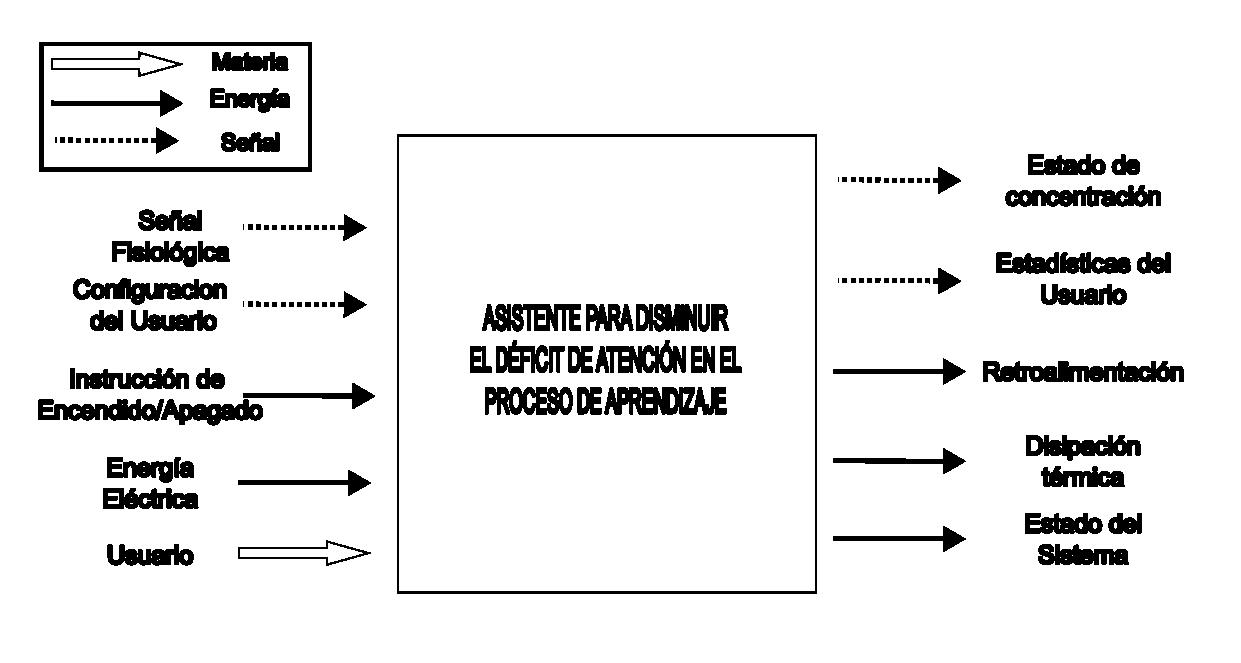
\includegraphics[width=0.73\textwidth]{CHPTRS/CH03_DICON/fig_cap3/Caja Negra.pdf}
\caption{Caja Negra del asistente}
\label{fig:caja negra}
\captionsetup{justification=centering,margin=2cm}
%\caption*{\textit{Elaboración propia}}
\end{figure}

A continuación se describen cada una de las entradas y salidas que se encuentran en la caja negra. No se consideraron flujos de materia, dado que el asistente no transforma ni intercambia sustancias físicas con el entorno o el usuario.\\

\hspace{-0.8cm}\underline{Entradas:}
\begin{itemize}
           
    \item Configuración del usuario: señal que indica la duración de la sesión de estudio y el inicio de su ejecución.
    \item Señal fisiológica: señal obtenida a partir del contacto físico con el usuario.
    \item Instrucción de Encendido/Apagado: acción que realiza el usuario para encender o apagar el asistente. 
    \item Energía eléctrica: energía suministrada por una fuente recargable, que permite el funcionamiento continuo del asistente.
    \item Usuario: estudiante que hará uso del asistente, encargado de ajustar su posicionamiento para el correcto funcionamiento.

         
\end{itemize}
\underline{Salidas:}
    
\begin{itemize}
    \item Estado de concentración: señal que indica si el usuario esta concentrado o no.
    \item Estadísticas del usuario: señal transmitida en el aplicativo que contiene métricas como porcentaje de concentración y el historial de sesiones.
    \item Retroalimentación: Energía emitida que retroalimenta al usuario en caso de que se encuentre en estado de desconcentración.
    \item Disipación térmica: Energía térmica liberada por los componentes electrónicos del asistente durante su funcionamiento, el encendido y el apagado del asistente.
    \item Estado del sistema: Indicador visual/sonoro que muestra si el asistente se encuentra encendido o apagado.
\end{itemize}


%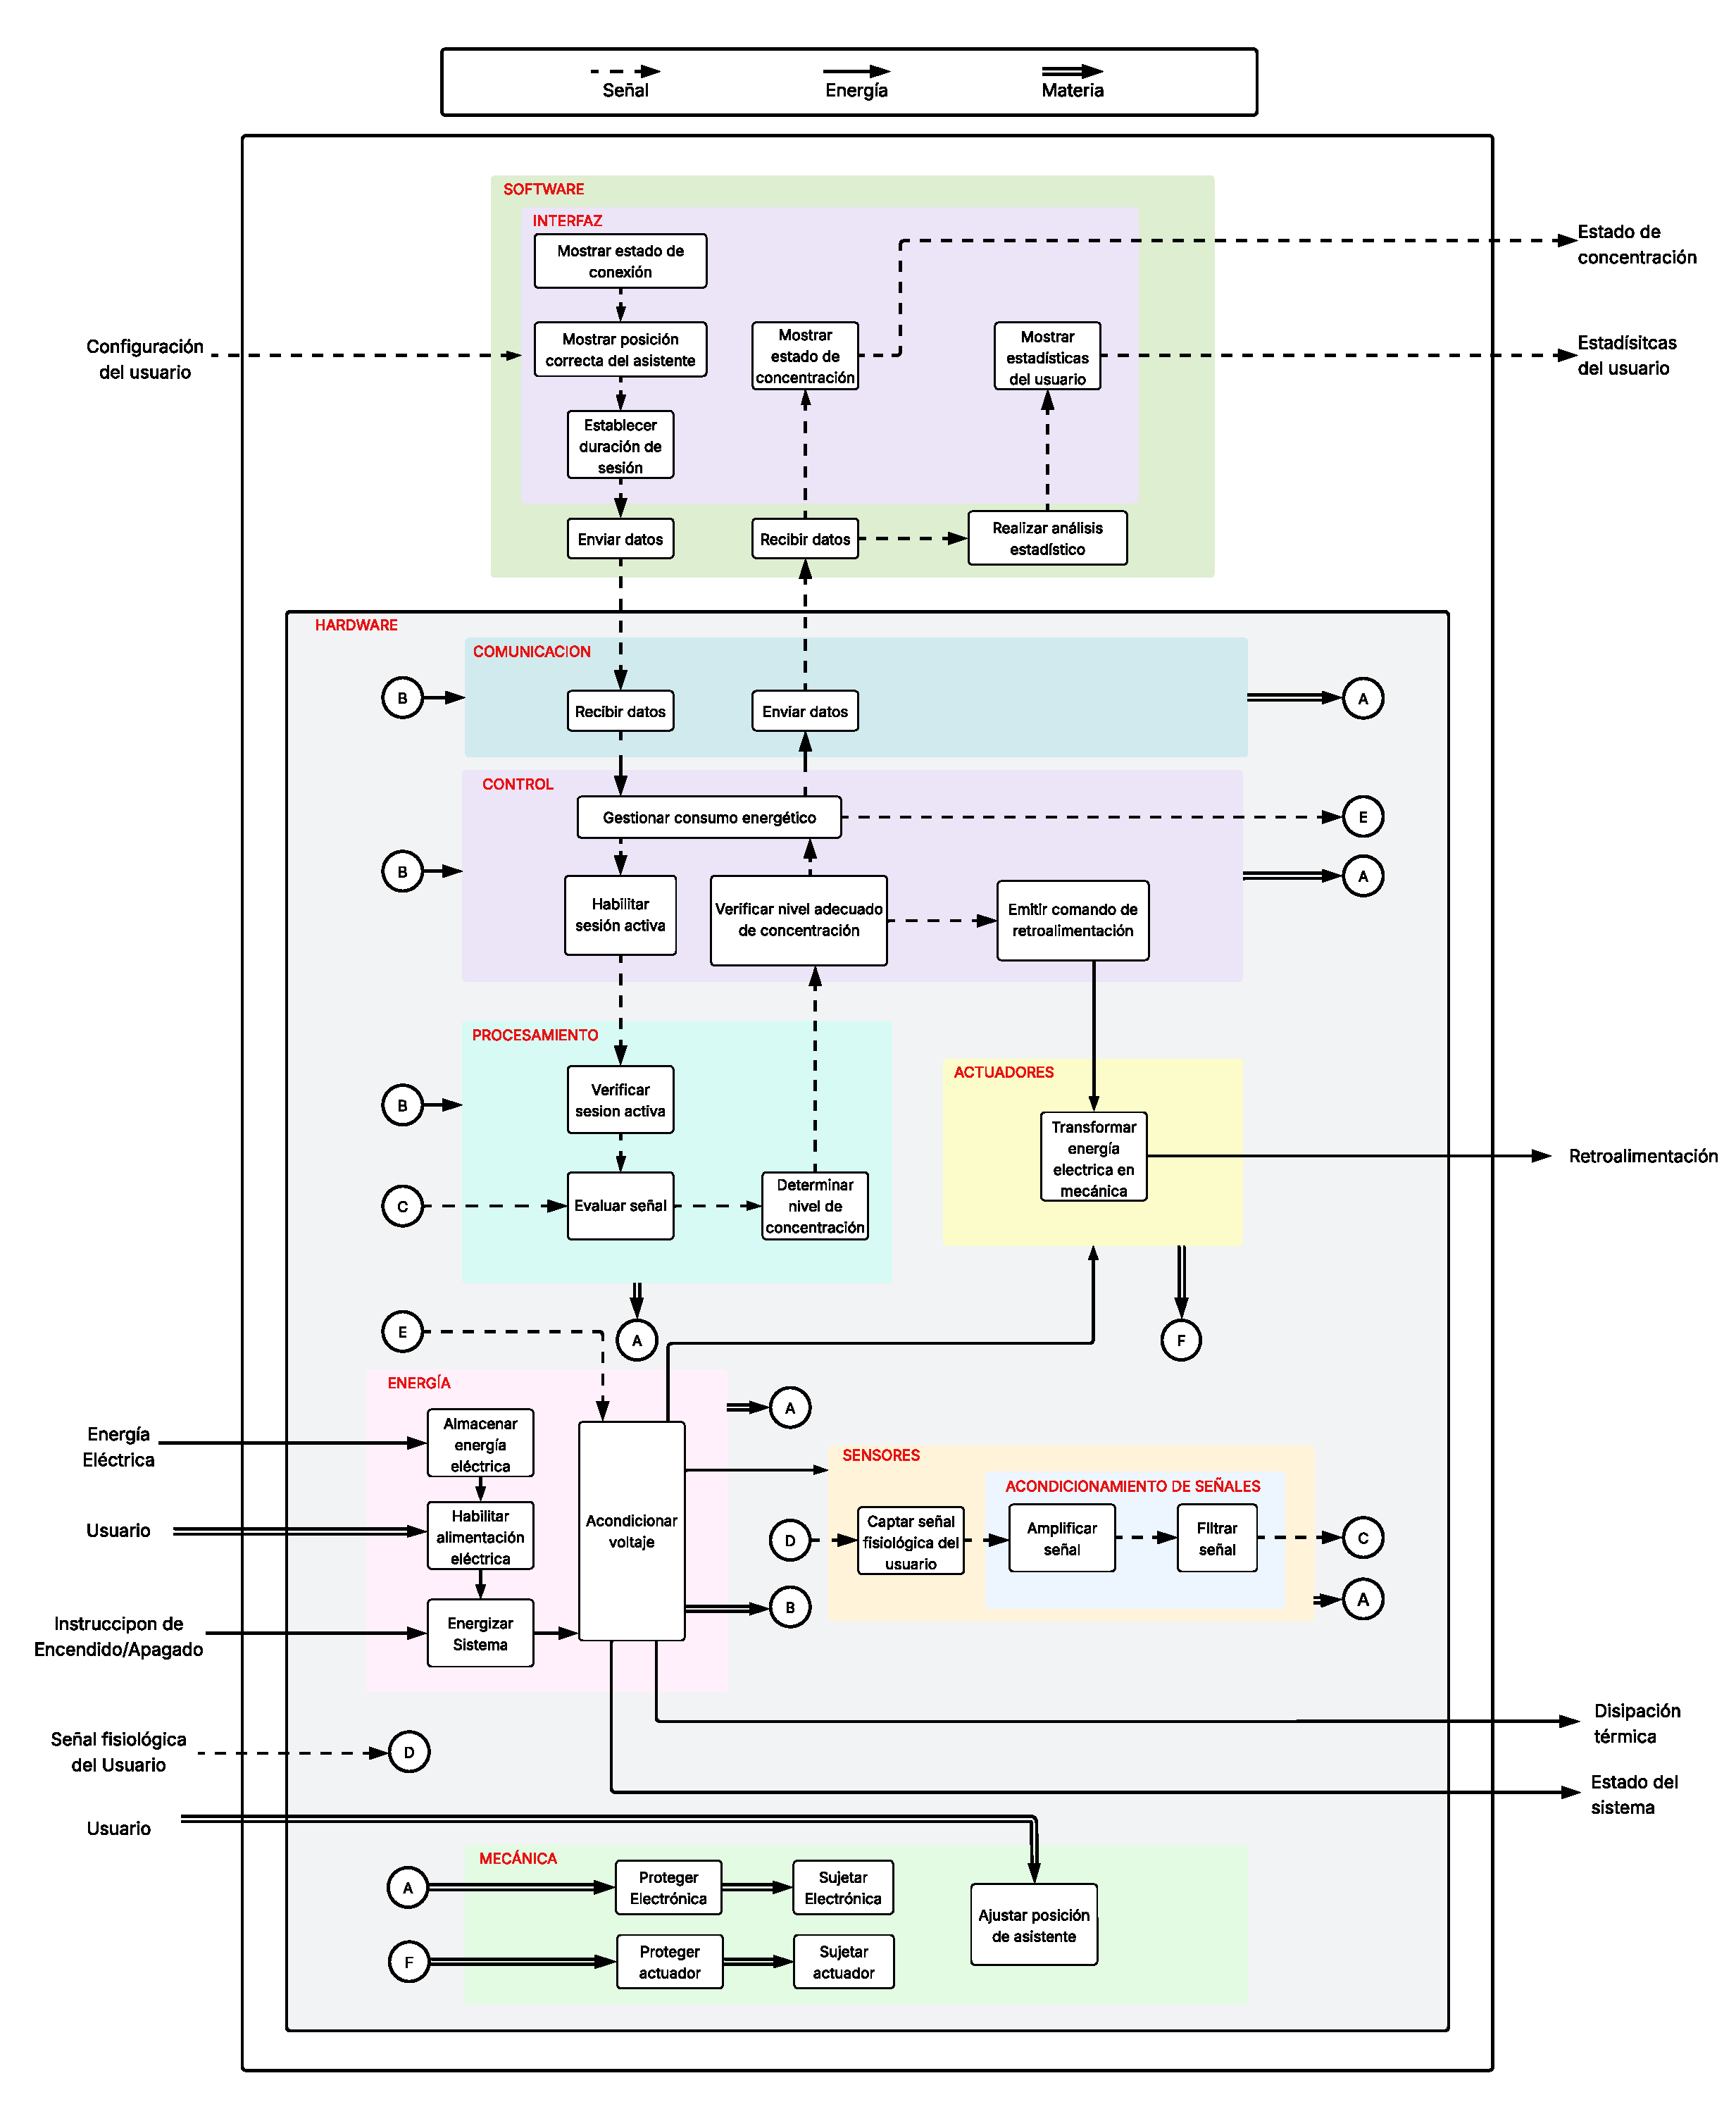
\includepdf[
 %   pages=1,
  %  pagecommand={},
   % fitpaper=true,
   % height=\textheight,
   % keepaspectratio  % Mantiene la relación de aspecto
%]{CHPTRS/CH03_DICON/fig_cap3/Estructura de funciones tesis.pdf}

%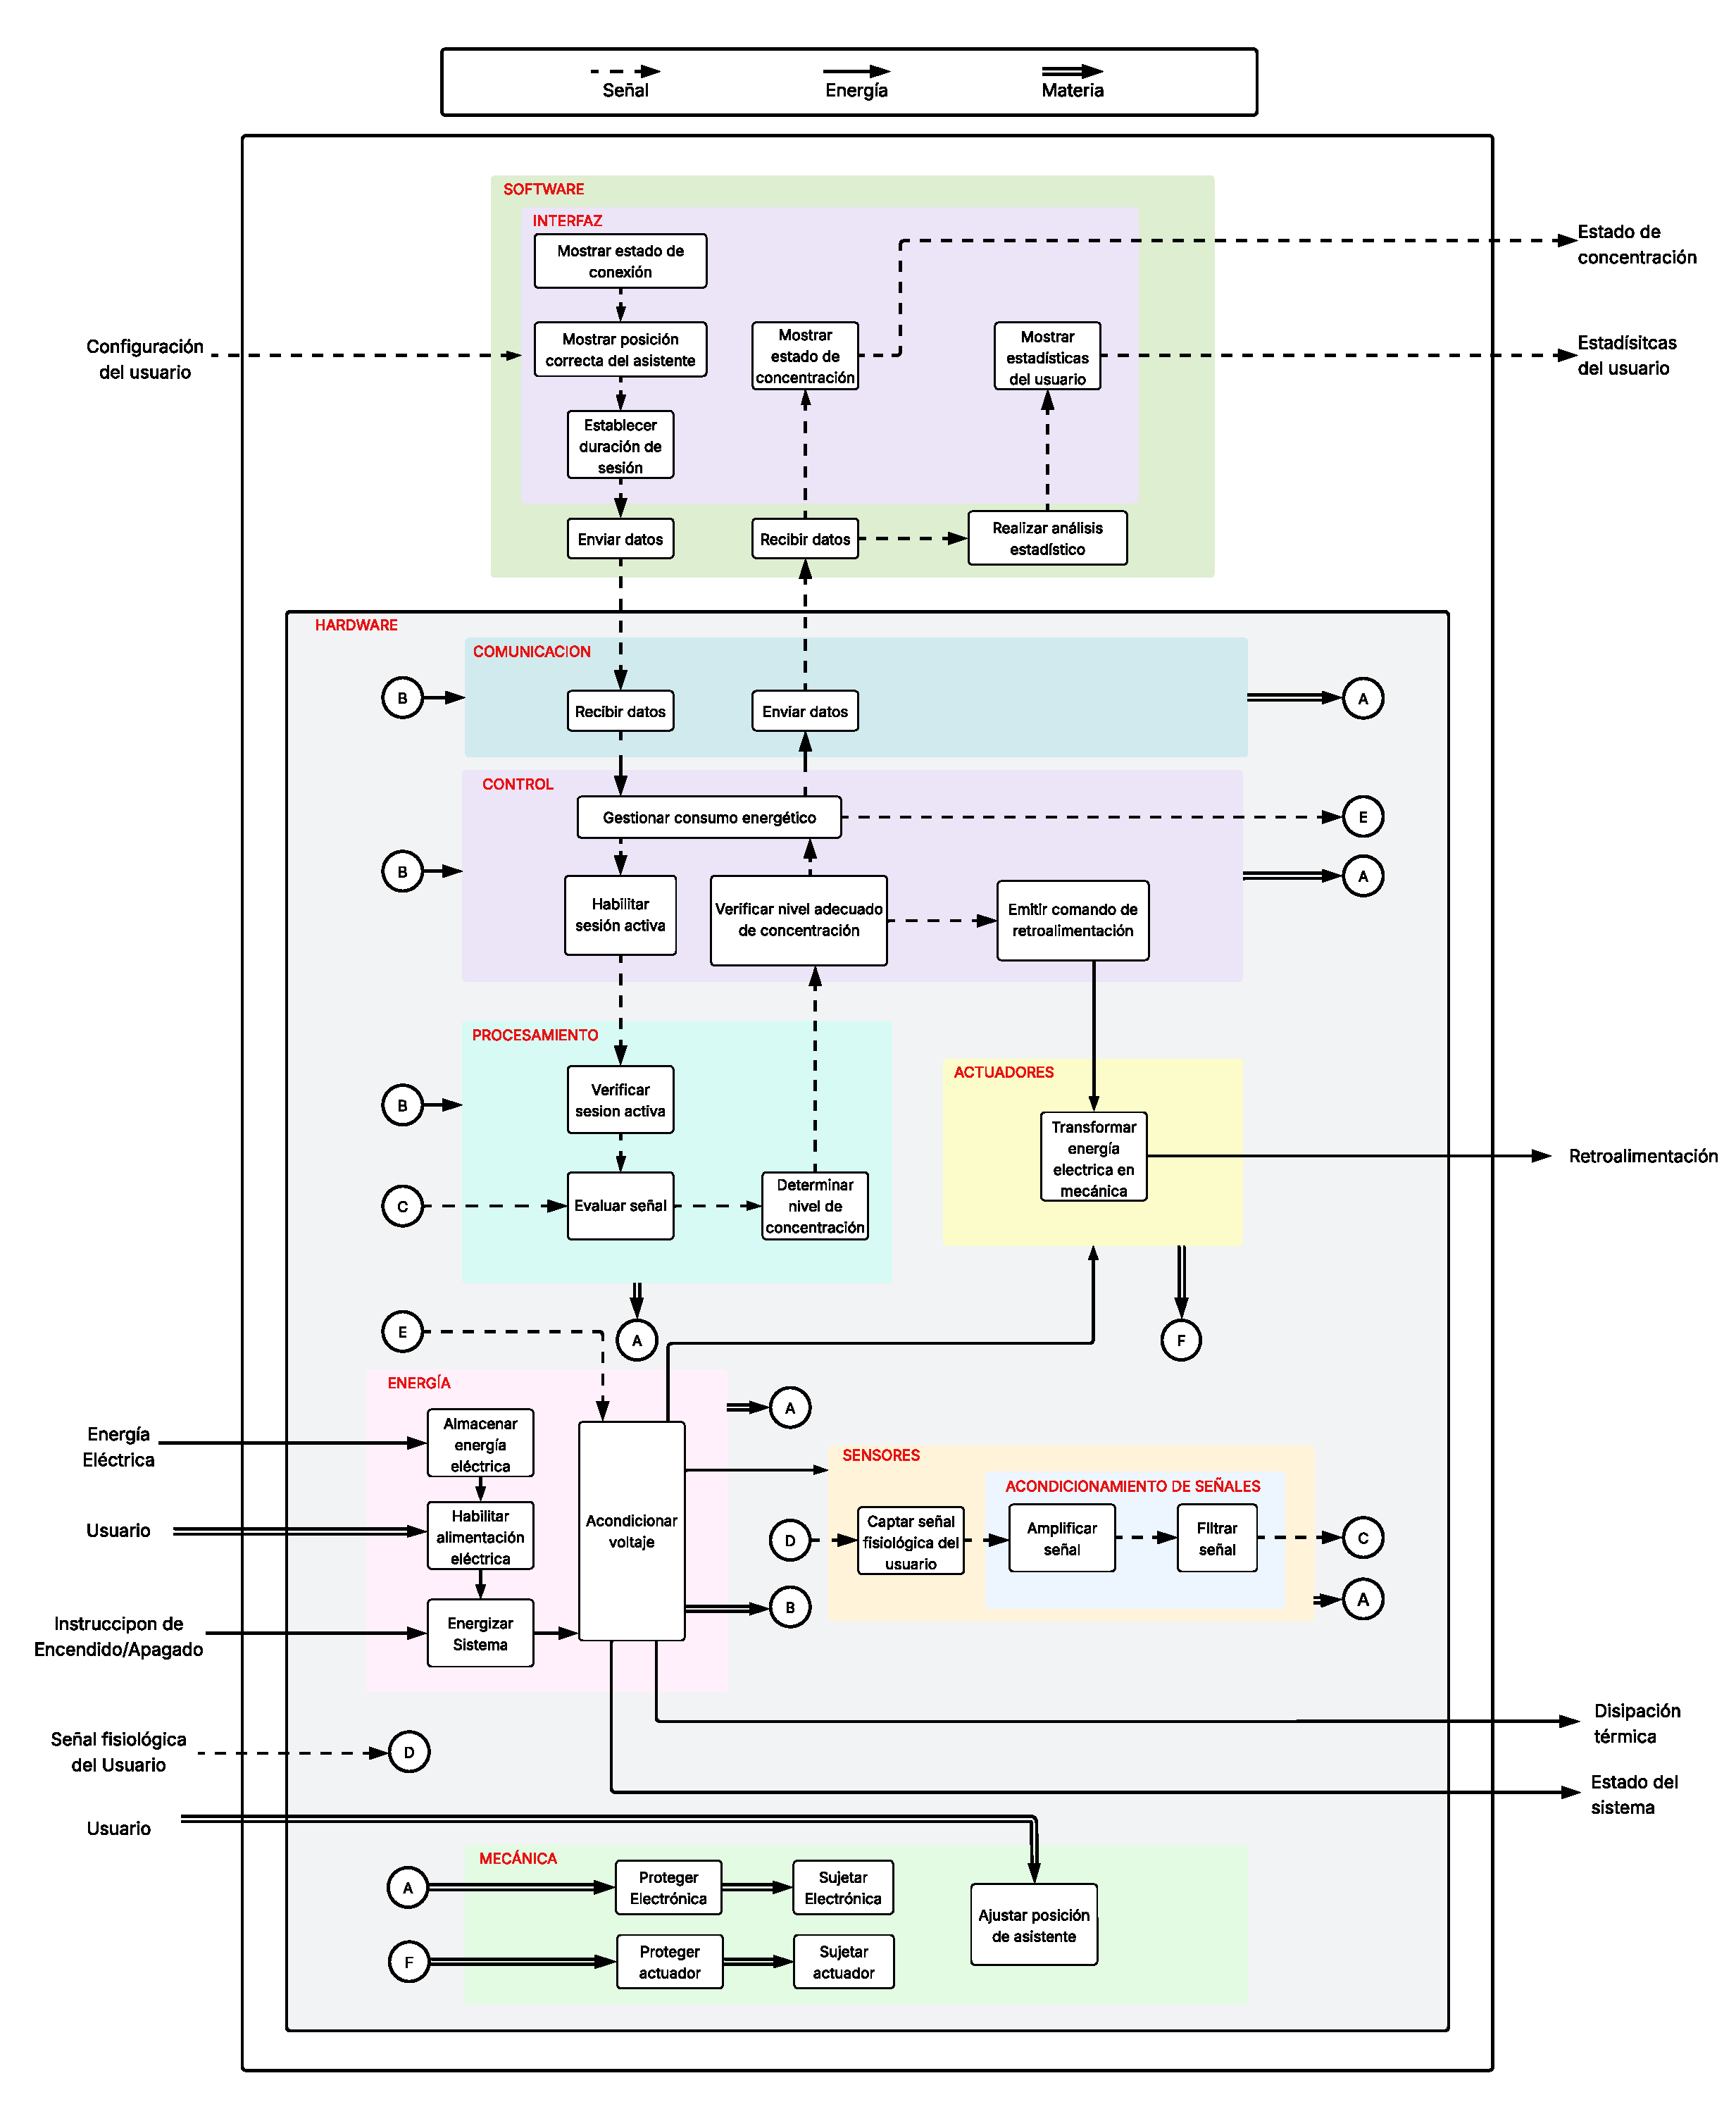
\includepdf[pages=-, pagecommand={}, width=\paperwidth, height=\paperheight]{CHPTRS/CH03_DICON/fig_cap3/Estructura de funciones tesis.pdf}





\subsection{Dominio Mecánico}
En el presente dominio, que se encuentra en la  Figura ~\ref{fig:d.mecanico}, se describen las funciones mecánicas necesarias para el funcionamiento del sistema. Este dominio se compone de 5 bloques funcionales. En primer lugar, se tiene las funciones de proteger electrónica y proteger actuador, cuyas funciones es resguardar los bloques funcionales internos de todos los otros dominios frente a golpes, polvo y otros agentes externos. Dado que esos componentes están integrados dentro de la estructura, ambos garantizan su durabilidad y correcto aislamiento.\\

Luego, se tiene a las funciones sujetar electrónica y sujetar actuador, las cuales buscan mantener en posición todos los elementos internos del asistente. De esta manera, asegura la estabilidad mecánica ante movimientos bruscos del usuario y facilita la conexión estructural entre los diversos componentes. Finalmente, la función ajustar posición de asistente, que depende de la acción del usuario, quien es el responsable de colocarlo sobre su cuerpo. Esta interacción permite garantizar un adecuado posicionamiento, necesario para asegurar el funcionamiento del asistente.
\begin{figure}[H]
\centering
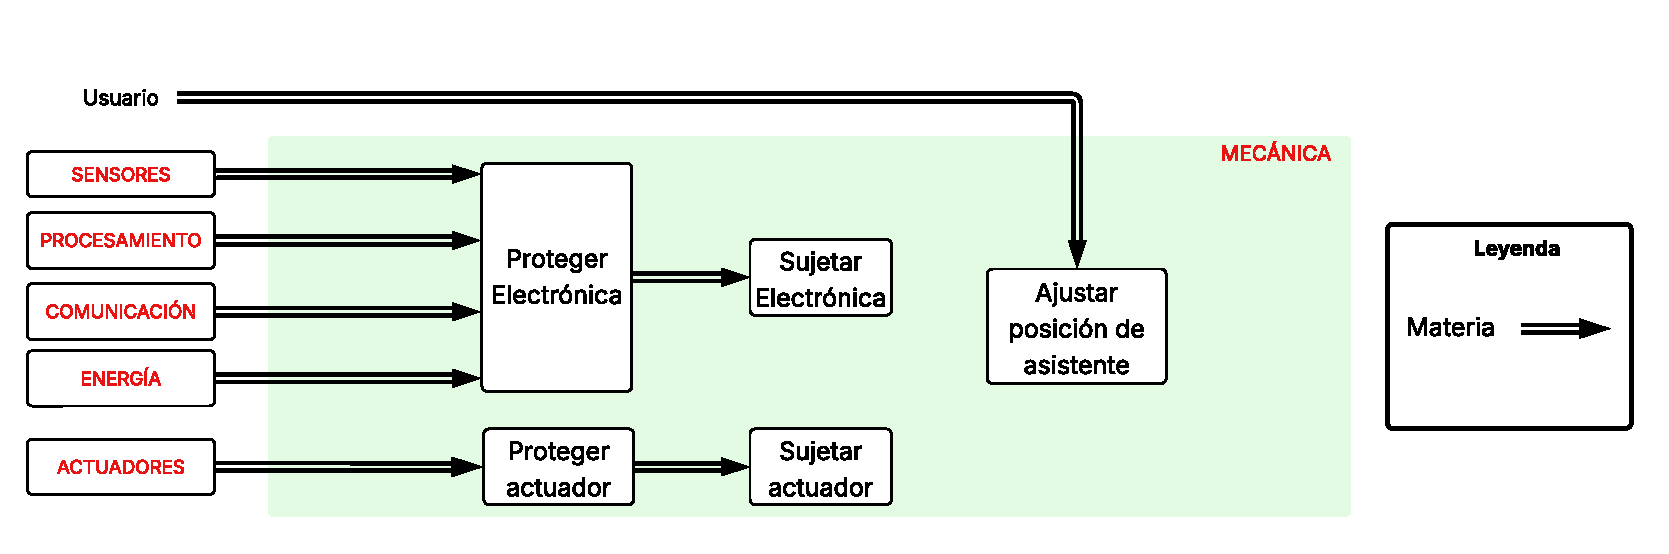
\includegraphics[width=0.9\textwidth]{CHPTRS/CH03_DICON/fig_cap3/Dominio mecánico.pdf}
\caption{Dominio mecánico del asistente}
\label{fig:d.mecanico}
\captionsetup{justification=centering,margin=2cm}
%\caption*{\textit{Elaboración propia}}
\end{figure}

\subsection{Dominio Energía}
El dominio energía tiene como finalidad asegurar el suministro energético continuo del asistente. Este está compuesto por tres funciones principales como se puedo apreciar en la Figura ~\ref{fig:d.energia}. La primera función es almacenar energía eléctrica que representa el componente encargado de contener la energía proveniente de la entrada energía eléctrica. La segunda es habilitar alimentación eléctrica, la cual depende de la instrucción de encendido o apagado realizada por el usuario.\\

Asimismo, la función energizar el sistema gestiona el flujo energético y la función acondicionar voltaje se encarga de regular la energía almacenada para que sea compatible con los requerimientos eléctricos de los distintos dominios (control, sensores, actuadores, comunicación y procesamiento). Esta función emite una señal de estado del sistema y su operación genera la salida de disipación térmica.Además, recibe una señal del dominio control en caso de que se requiera colocar el asistente en modo de bajo consumo. Finalmente, dado que los componentes forman parte del hardware del asistente, el dominio energía se encuentra estructuralmente integrado dentro de la protección mecánica del asistente.    

\begin{figure}[H]
\centering
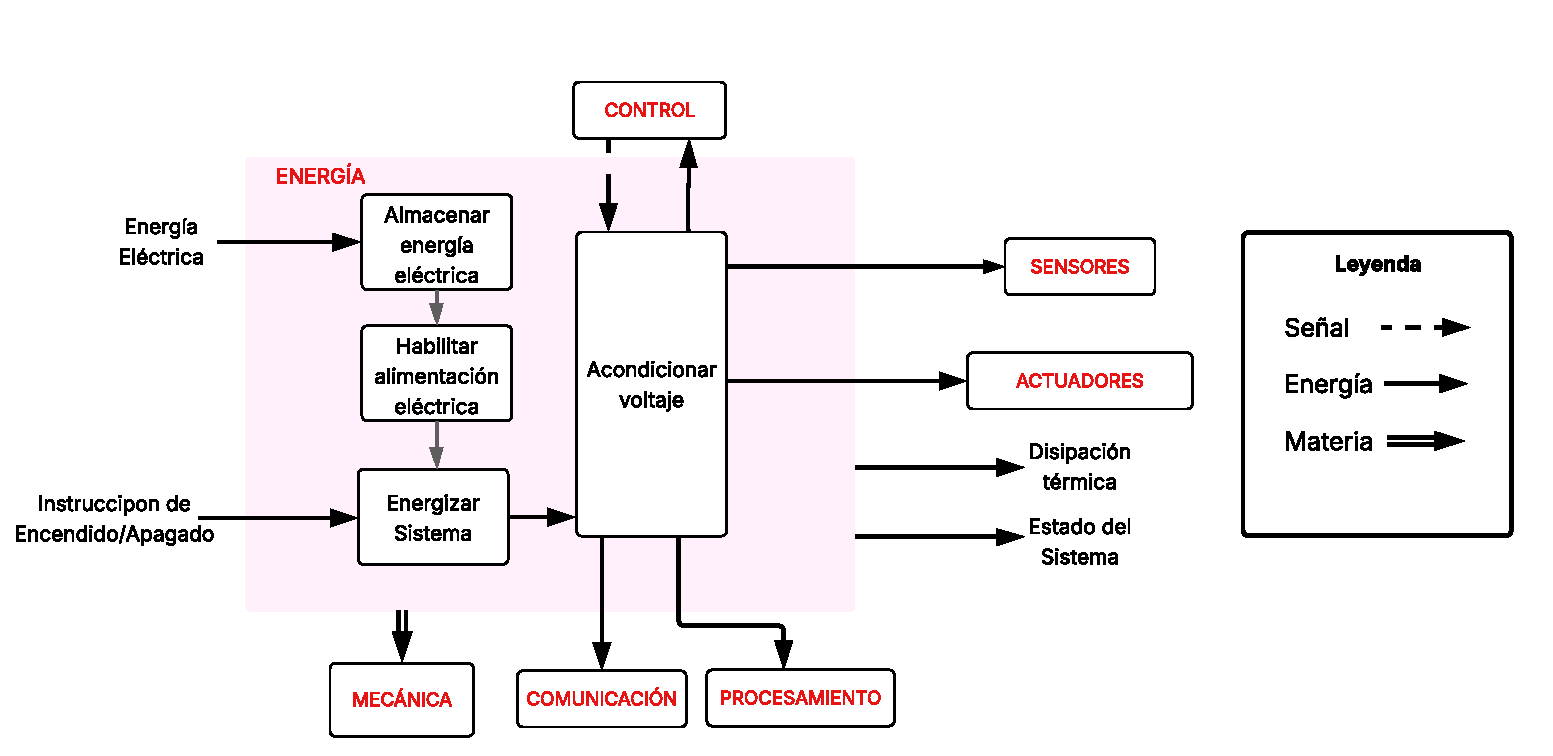
\includegraphics[width=0.9\textwidth]{CHPTRS/CH03_DICON/fig_cap3/Dominio Energia.pdf}
\caption{Dominio energía del asistente}
\label{fig:d.energia}
\captionsetup{justification=centering,margin=2cm}
%\caption*{\textit{Elaboración propia}}
\end{figure}

\subsection{Dominio Sensores}
El dominio sensores tiene como finalidad captar y acondicionar la señal fisiológica del usuario, permitiendo la posterior evaluación del estado de concentración (ver Figura ~\ref{fig:d.sensores}). Cabe señalar que el tipo específico de señal fisiológica a utilizar será definido en función de las alternativas tecnológicas evaluadas en las matrices morfológicas presentadas en la siguiente sección. Además, el funcionamiento del presente dominio depende directamente del suministro de energía eléctrica proporcionada por el dominio energía.\\

La primera función es captar señal fisiológica del usuario, habilitada por el contacto físico proporcionado por la estructura mecánica. Posteriormente, se tiene un subdominio acondicionamiento de señales donde se busca amplificar la señal para facilitar su tratamiento y finalmente la función filtrar señal que elimina interferencias y ruidos no deseados, asegurando que solo la información relevante llegue al dominio de procesamiento. 



\begin{figure}[H]
\centering
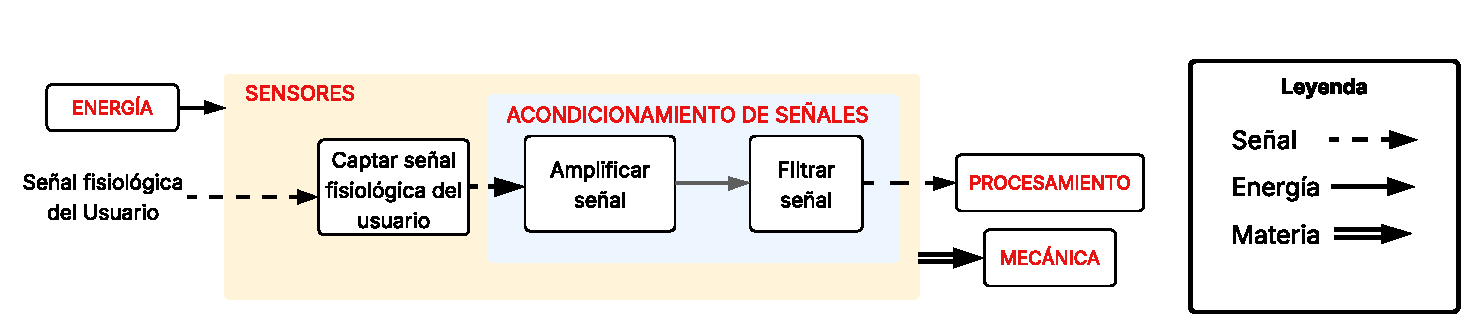
\includegraphics[width=0.9\textwidth]{CHPTRS/CH03_DICON/fig_cap3/Dominio Sensores.pdf}
\caption{Dominio sensores del asistente}
\label{fig:d.sensores}
\captionsetup{justification=centering,margin=2cm}
%\caption*{\textit{Elaboración propia}}
\end{figure}



%\subsection{Dominio Acondicionamiento de Señales}
%El presente dominio (ver Figura %%~\ref{fig:d.acondicionamiento}) tiene como funciones %%principales la amplificación de la señal obtenida del dominio sensores. Posteriormente,  se filtra con el objetivo de eliminar el ruido y las interferencias para ser enviada al dominio procesamiento en las mejores condiciones para su análisis.

%\begin{figure}[H]
%%\centering
%\includegraphics[width=0.5\textwidth]%{CHPTRS/CH03_DICON/fig_cap3/Dominio Acondicionamiento.pdf}
%\caption{Dominio Acondicionamiento de Señales del asistente}
%\label{fig:d.acondicionamiento}
%\captionsetup{justification=centering,margin=2cm}
%\caption*{\textit{Elaboración propia}}
%\end{figure}

\subsection{Dominio Procesamiento}

El dominio procesamiento, que se encuentra en la Figura ~\ref{fig:d.procesamiento}, se encarga de analizar la señal fisiológica acondicionada por el dominio sensores a través de ciertas funciones interconectadas. La primera de ellas es verificar sesión activa, la cual valida si existe una sesión de estudio en curso a partir de la señal de control proveniente del dominio control. Luego, la función evaluar señal analiza las características de la señal fisiológica con el objetivo de extraer indicadores relevantes de atención unicamente si la sesión esta activa. Esta información es utilizada por la función determinar el nivel de concentración del usuario, en si se encuentra en estado de concentración o distracción. Asimismo, el resultado es transmitido al dominio control, el cual se encarga de decidir la acción correspondiente. Este dominio requiere de alimentación eléctrica proveniente del dominio energía para su funcionamiento, y sus componentes físicos se encuentran contenidos dentro del dominio mecánico. 

\begin{figure}[H]
\centering
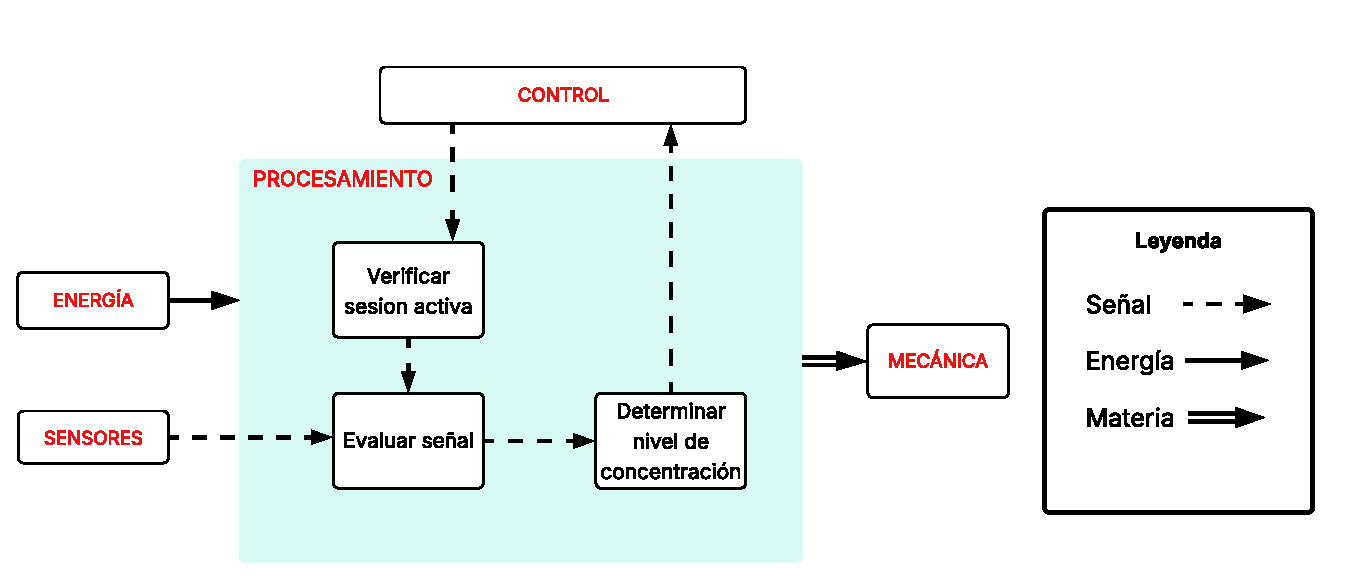
\includegraphics[width=0.8\textwidth]{CHPTRS/CH03_DICON/fig_cap3/Dominio procesamiento.pdf}
\caption{Dominio procesamiento del asistente}
\label{fig:d.procesamiento}
\captionsetup{justification=centering,margin=2cm}
%\caption*{\textit{Elaboración propia}}
\end{figure}

 


\subsection{Dominio Control}

El presente dominio control se encarga de coordinar el comportamiento lógico del asistente tomando decisiones. Esto se realiza a partir de los datos obtenidos de los dominios comunicación y procesamiento como se puede apreciar en la Figura ~\ref{fig:d.control}).\\

La función gestionar consumo energético se encarga de verificar si se esta haciendo uso del asistente. En caso contrario, manda una señal al dominio energía para acondicionar el voltaje y establecer el sistema en modo bajo consumo. Luego, el bloque habilitar sesión activa gestiona la activación de la sesión de estudio, permitiendo que el procesamiento de la señal fisiológica se realice únicamente durante las sesiones de estudio.\\

Además, la función verificar nivel adecuado de concentración analiza el si el nivel de concentración determinado en el dominio procesamiento es adecuado. En caso contrario, se emite el comando de retroalimentación. Este dominio requiere energía eléctrica del dominio energía, y sus componentes físicos forman parte de la estructura del asistente. 

\begin{figure}[H]
\centering
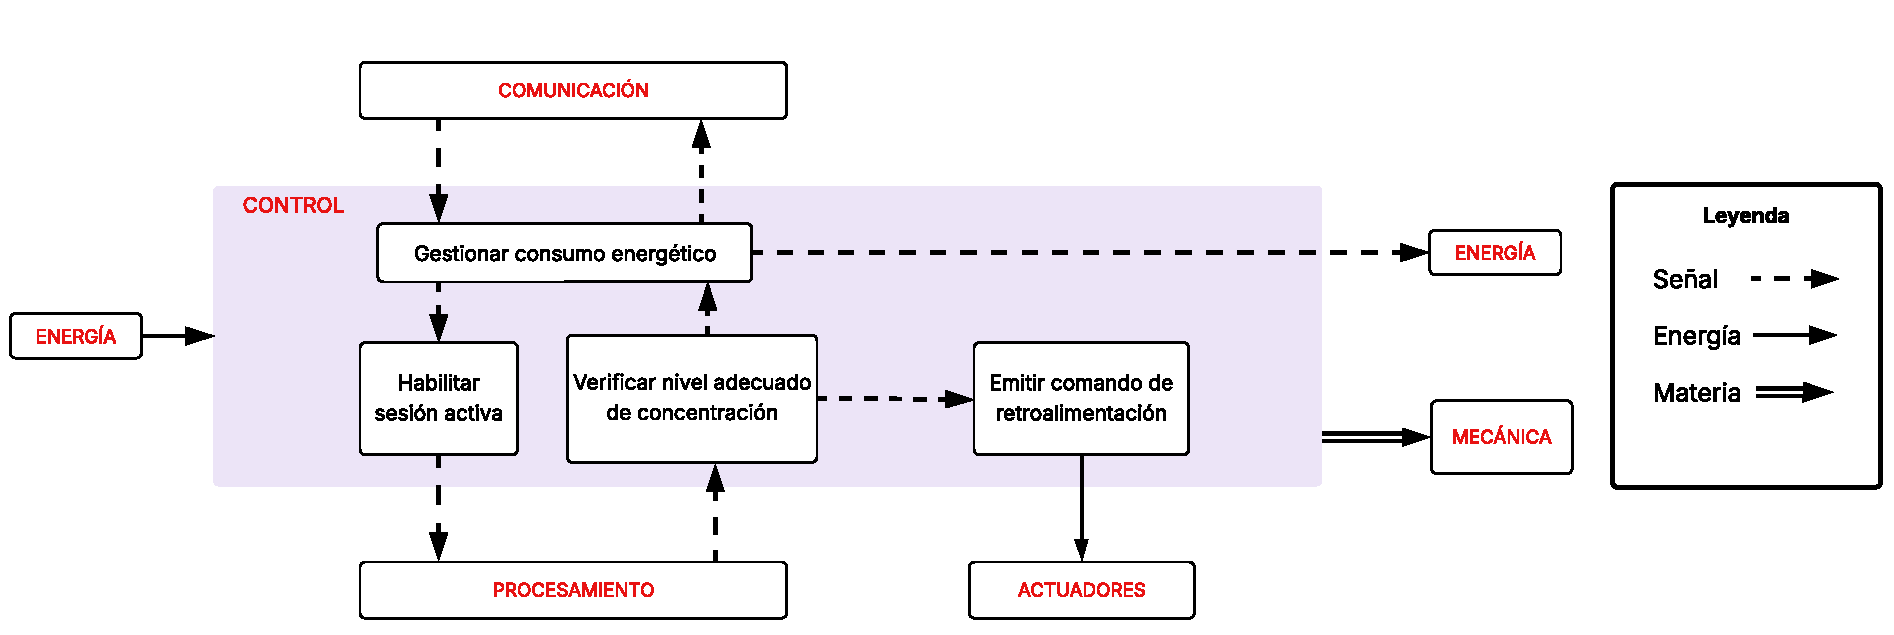
\includegraphics[width=1\textwidth]{CHPTRS/CH03_DICON/fig_cap3/Dominio control.pdf}
\caption{Dominio control del asistente}
\label{fig:d.control}
\captionsetup{justification=centering,margin=2cm}
%\caption*{\textit{Elaboración propia}}
\end{figure}

\subsection{Dominio Comunicación}
El dominio de comunicación (ver Figura ~\ref{fig:d.comuninación}) permite el intercambio de información entre el asistente y el \ac{SW} o aplicativo del sistema, actuando como puente entre los procesos internos y la interfaz externa del usuario. La primera función, recibir datos, se encarga de captar la información del dominio de control (los estados de concentración y el consumo energético) y del dominio \ac{SW} (duración de la sesión). Asimismo, la función enviar datos transmite tanto al dominio \ac{SW}  como al dominio comunicación los datos mencionados previamente y también los casos donde se detecte que no se encuentra una sesión activa para que el dominio control pueda gestionar el consumo energético. El domino opera bajo soporte energético proveniente del dominio energía y sus componentes físicos se encuentran en el dominio mecánico.\\

\begin{figure}[H]
\centering
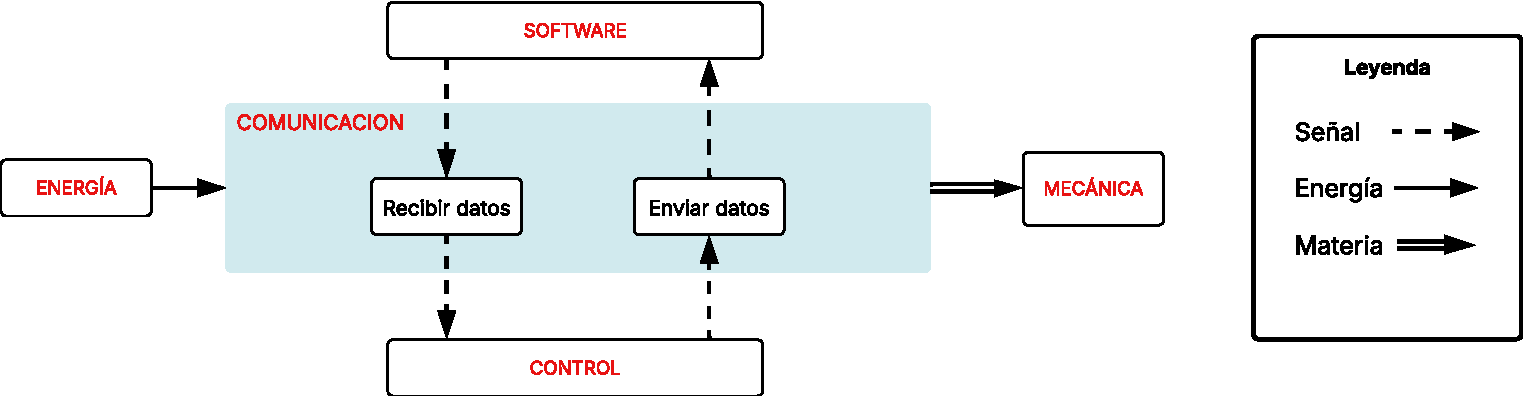
\includegraphics[width=0.85\textwidth]{CHPTRS/CH03_DICON/fig_cap3/Dominio comunicación.pdf}
\caption{Dominio comunicación del asistente}
\label{fig:d.comuninación}
\captionsetup{justification=centering,margin=2cm}
%\caption*{\textit{Elaboración propia}}
\end{figure}

\subsection{Dominio Actuadores}
La retroalimentación del asistente se lleva a cabo mediante la función de transformar la energía eléctrica en energía mecánica a través de un actuador, generando la retroalimentación al usuario (ver Figura~\ref{fig:d.retroalimentación}). Esta se activa a partir de la señal proveniente del dominio control que establece si el usuario esta concentrado o distraído. El actuador se encuentra integrado al asistente, cuya presencia se encuentra dentro de la estructura del dominio mecánico.

\begin{figure}[H]
\centering
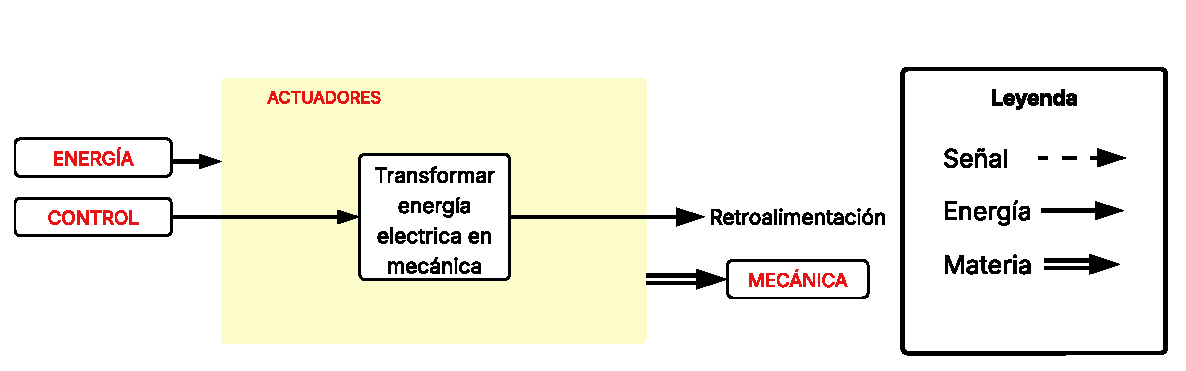
\includegraphics[width=0.8\textwidth]{CHPTRS/CH03_DICON/fig_cap3/Dominio retroalimentación.pdf}
\caption{Dominio retroalimentación del asistente}
\label{fig:d.retroalimentación}
\captionsetup{justification=centering,margin=2cm}
%\caption*{\textit{Elaboración propia}}
\end{figure}

\subsection{Dominio Software}

El dominio \ac{SW} representa al aplicativo mediante el cual el usuario interactúa con el asistente. Está compuesto por funciones que permiten tanto la comunicación con el asistente como la visualización de información mediante funciones que forman parte del subdominio interfaz, como se puede aprecia en la Figura~\ref{fig:d.software}). A través de la interfaz, el usuario puede realizar su configuración y establecer la duración de sesión de estudio, generando la señal de configuración que es transmitida al asistente mediante la función enviar datos.  \\

Por otro lado, los datos recibidos por el sistema son procesados mediante la función realizar análisis estadístico, y los resultados se visualizan en la interfaz mediante las funciones mostrar estado de concentración y mostrar estadísticas del usuario, así como  el estado de conexión con el asistente. Estas funciones constituyen las salidas correspondientes del asistente (estado de concentración y estadísticas del usuario).

\begin{figure}[H]
\centering
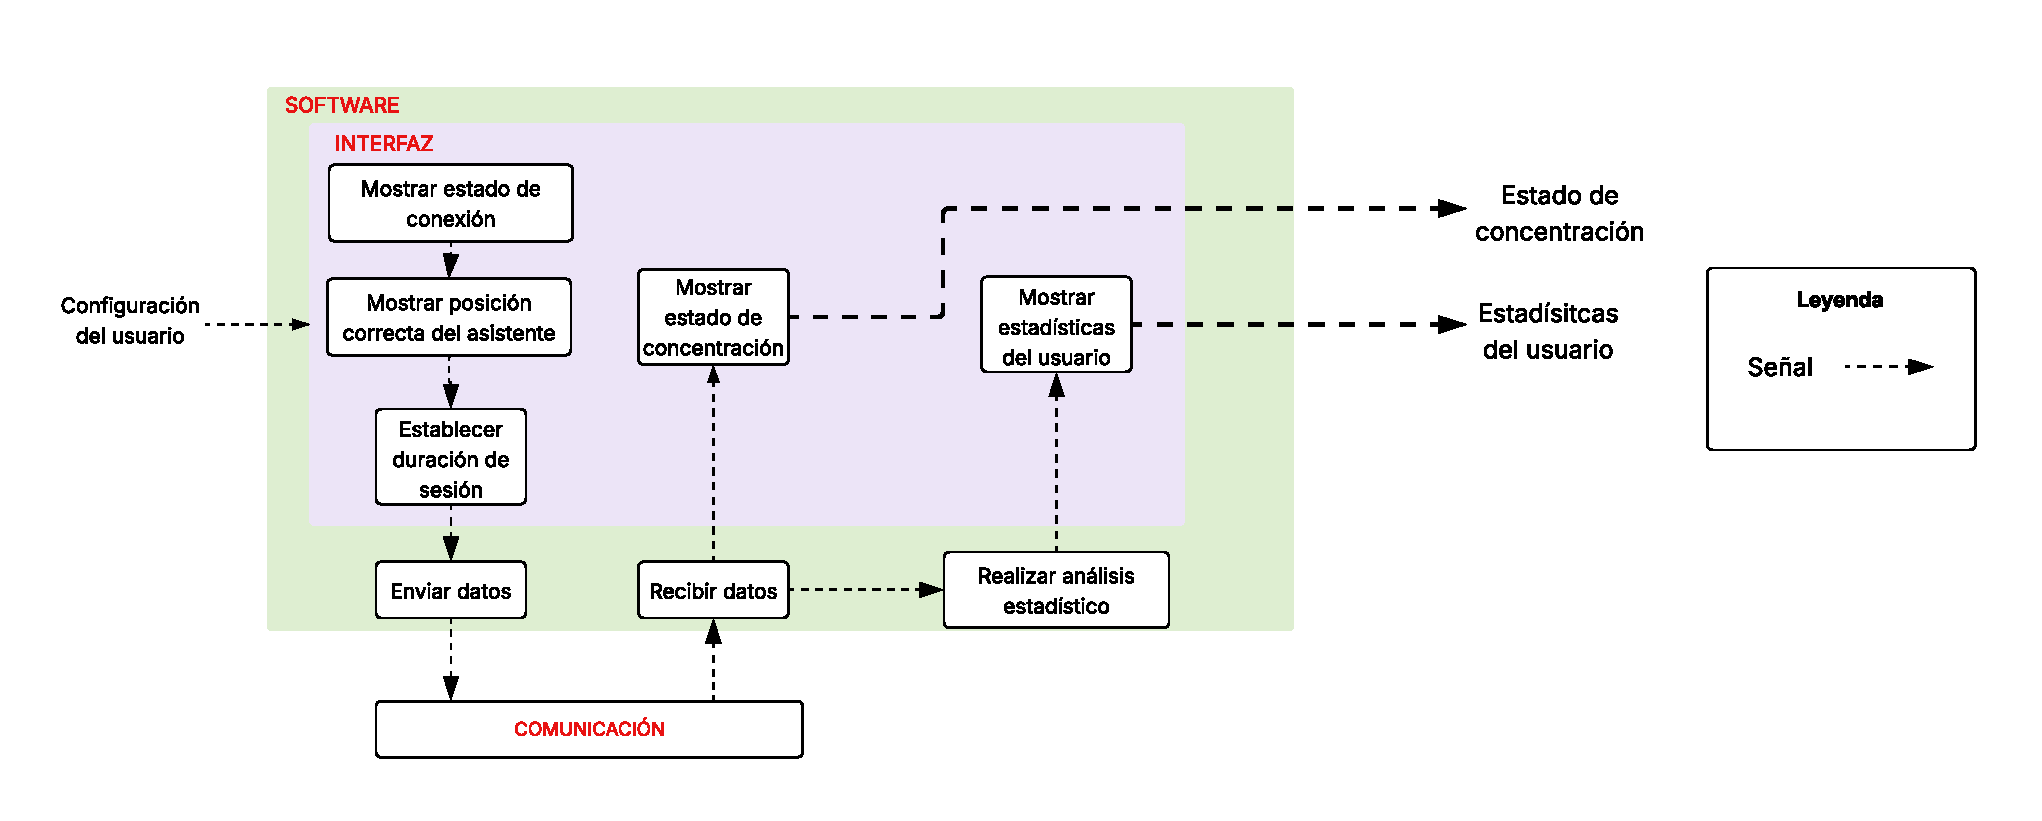
\includegraphics[width=0.95\textwidth]{CHPTRS/CH03_DICON/fig_cap3/Dominio software.pdf}
\caption{Dominio software del asistente}
\label{fig:d.software}
\captionsetup{justification=centering,margin=2cm}
%\caption*{\textit{Elaboración propia}}
\end{figure}


%\cleardoublepage 
%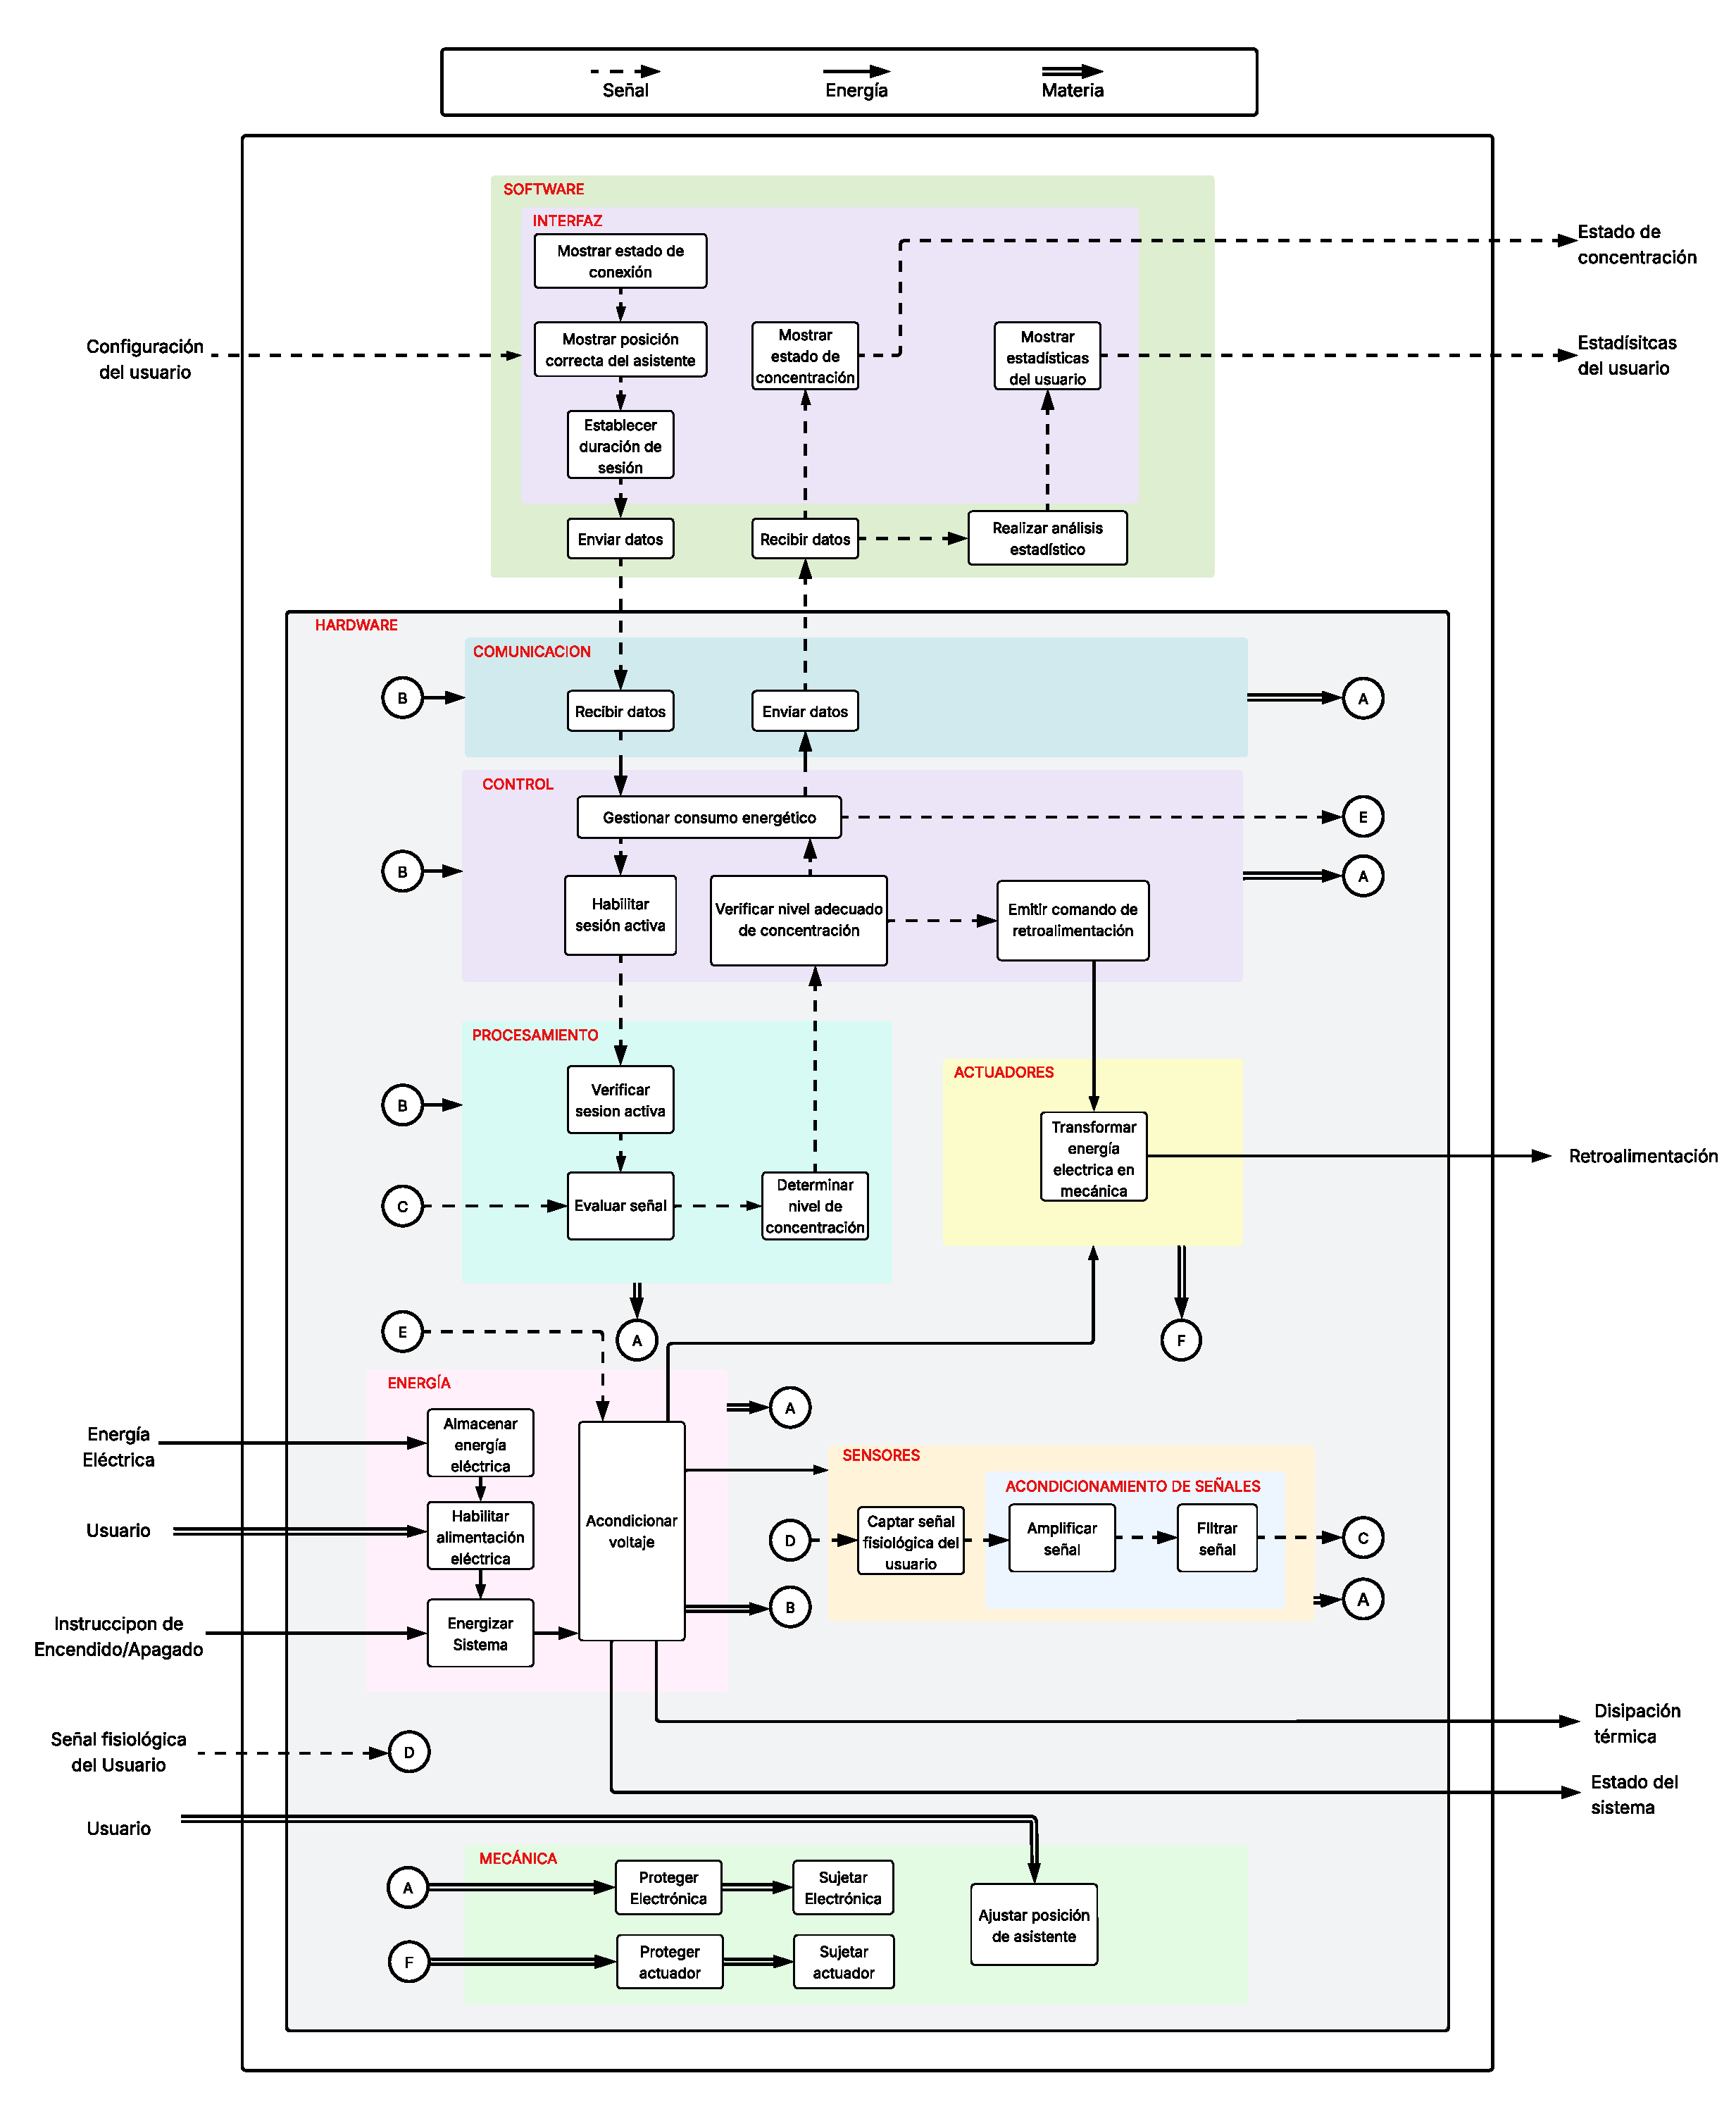
\includepdf[pages=1, pagecommand={}, fitpaper=false]{CHPTRS/CH03_DICON/fig_cap3/Estructura de funciones tesis.pdf}

%\cleardoublepage 
\section{Matriz morfológica}
La matriz morfológica permite evaluar diferentes soluciones técnicas para las funciones claves del asistente. Esta permite visualizar de forma estructurada el conjunto de posibles soluciones parciales, considerando en las opciones su viabilidad e integración entre componentes. A continuación, se presentará una matriz morfológica con diferentes alternativas por cada dominio explicado en la sección anterior con la finalidad de obtener 3 conceptos solución para el asistente, eligiendo una solución por cada función en la matriz.  Para ello, se tiene un color para cada  \ac{CoS} (ver Tabla~\ref{tab:leyendaConceptos}), donde las flechas de color rojo representa al primer \ac{CoS}, las flechas de color verde al segundo y las flechas azules al tercero. Los resultados de la combinación de las diferentes alternativas serán analizados en la siguiente \hyperref[sc:CH03-ev_tec-eco]{sección} mediante un análisis técnico-económico.


\begin{table}[H]
    \centering
    \caption{Leyenda de conceptos de solución}
    \label{tab:leyendaConceptos}
    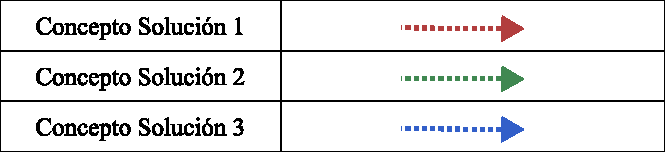
\includegraphics[width=0.6\textwidth]{CHPTRS/CH03_DICON/fig_matriz/FLECHAS.pdf}
\end{table}

\cleardoublepage

\begin{itemize}
\item{Matriz morfológica del dominio Software} 
\begin{table}[H]
    \centering
    \caption{Matriz morfológica del dominio Software}
    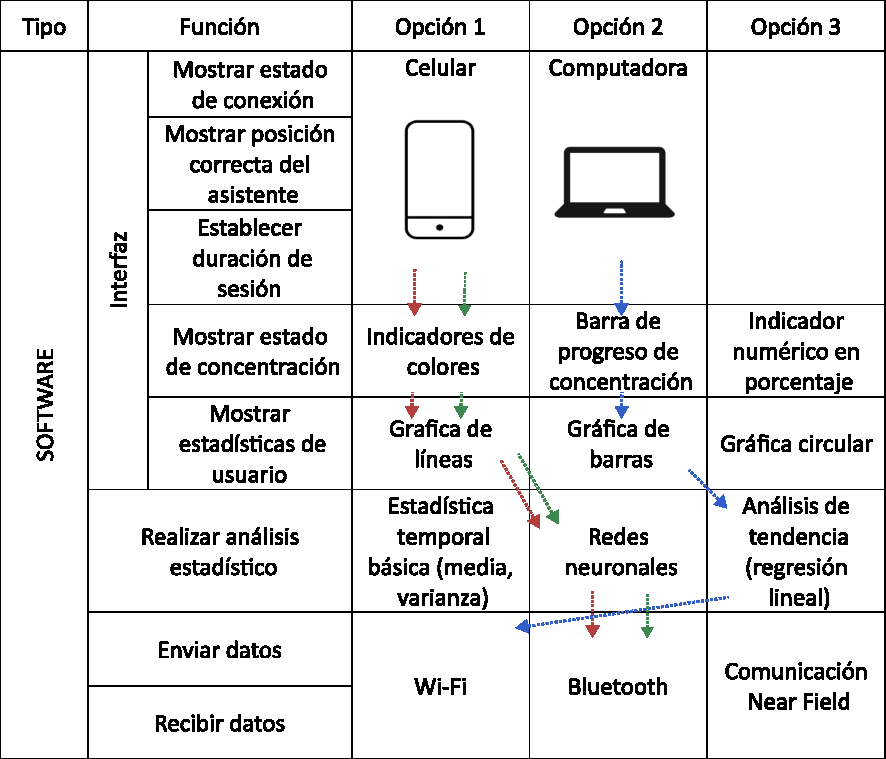
\includegraphics[width=0.8\textwidth]{CHPTRS/CH03_DICON/fig_matriz/Matriz software .pdf}
\end{table}

\item{Matriz morfológica del dominio Comunicación} 
\begin{table}[H]
    \centering
    \caption{Matriz morfológica del dominio Comunicación}
    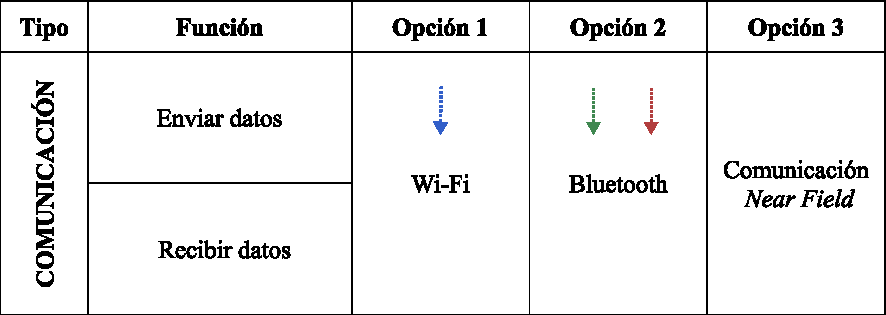
\includegraphics[width=0.8\textwidth]{CHPTRS/CH03_DICON/fig_matriz/Matriz comunicacion .pdf}
\end{table}


\item{Matriz morfológica del dominio Control} 

\begin{table}[H]
    \centering
    \caption{Matriz morfológica del dominio Control}
    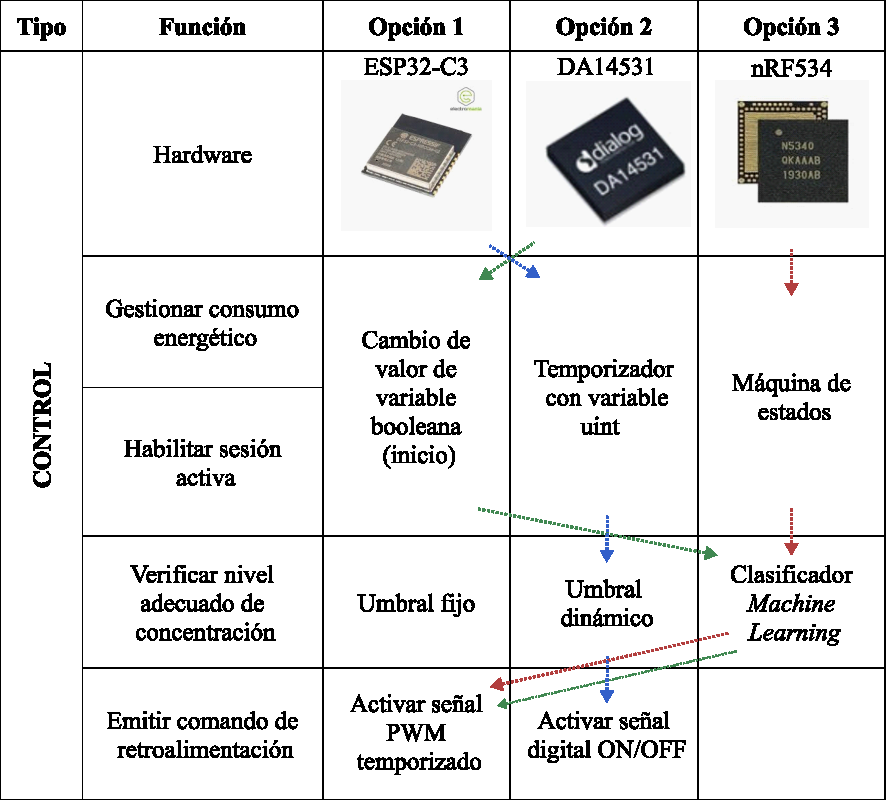
\includegraphics[width=0.8\textwidth]{CHPTRS/CH03_DICON/fig_matriz/Matriz control .pdf}
\end{table}
\item{Matriz morfológica del dominio Procesamiento} 

\begin{table}[H]
    \centering
    \caption{Matriz morfológica del dominio Procesamiento}
    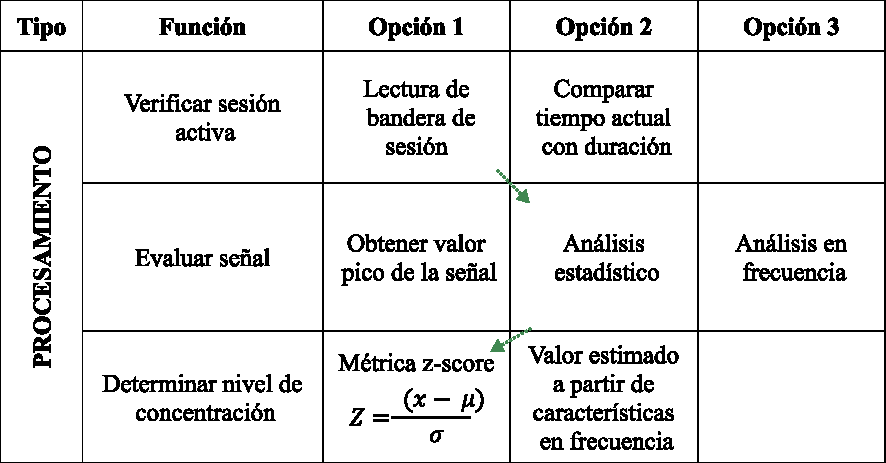
\includegraphics[width=0.8\textwidth]{CHPTRS/CH03_DICON/fig_matriz/Matriz procesamiento.pdf}
\end{table}
\item{Matriz morfológica del dominio Actuadores} 

\begin{table}[H]
    \centering
    \caption{Matriz morfológica del dominio Actuadores}
    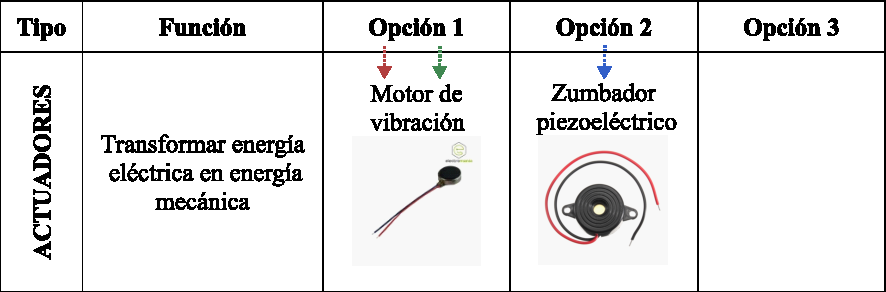
\includegraphics[width=0.8\textwidth]{CHPTRS/CH03_DICON/fig_matriz/Matriz actuadores .pdf}
\end{table}

\item{Matriz morfológica del dominio Energía} 
\begin{table}[H]
    \centering
    \caption{Matriz morfológica del dominio Energía}
    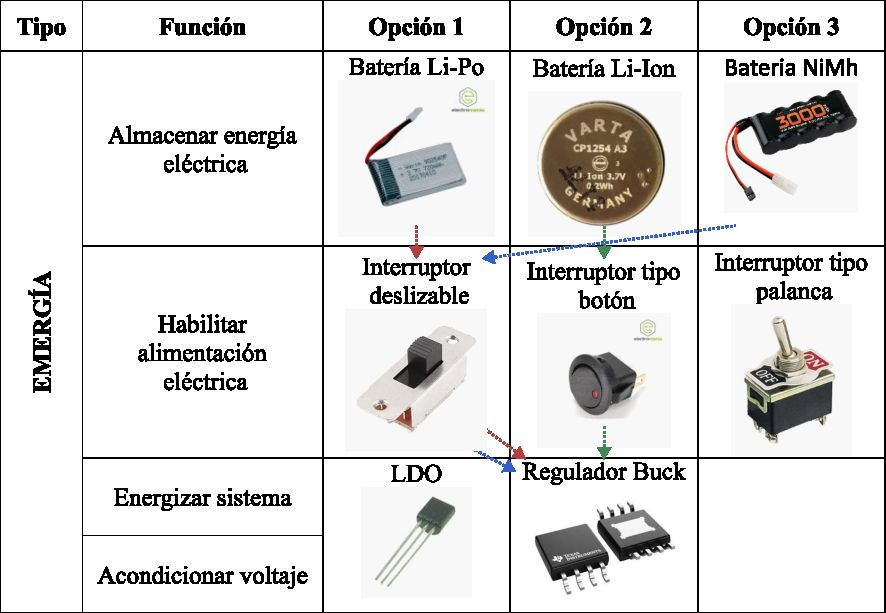
\includegraphics[width=0.8\textwidth]{CHPTRS/CH03_DICON/fig_matriz/Matriz energia.pdf}
\end{table}
\cleardoublepage

\item{Matriz morfológica del dominio Sensores} 
\begin{table}[H]
    \centering
    \caption{Matriz morfológica del dominio Sensores}
    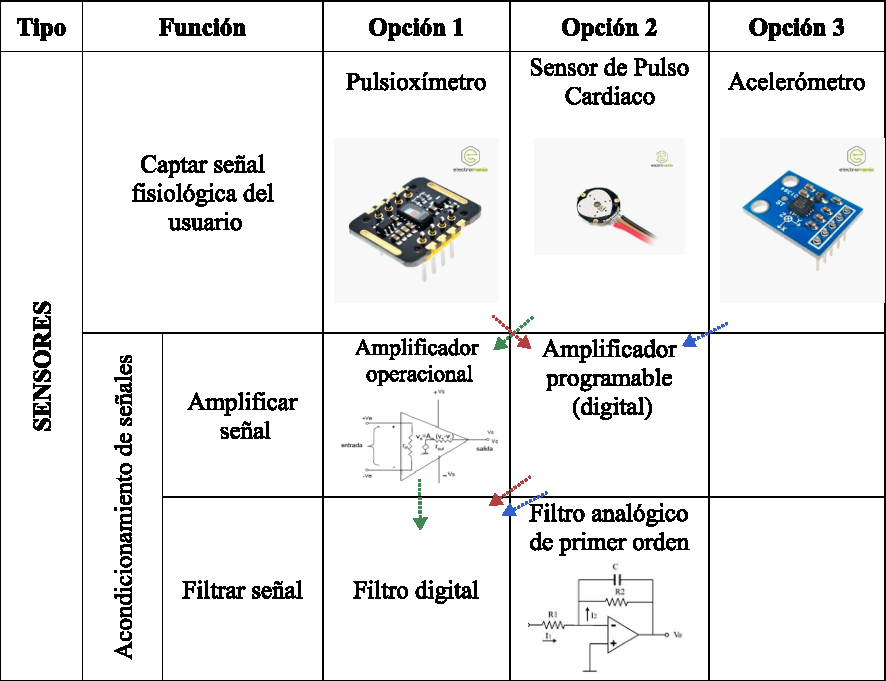
\includegraphics[width=0.8\textwidth]{CHPTRS/CH03_DICON/fig_matriz/Matriz sensores .pdf}
\end{table}
\cleardoublepage

\item{Matriz morfológica del dominio Mecánica} 
\begin{table}[H]
    \centering
    \caption{Matriz morfológica del dominio Mecánica}
    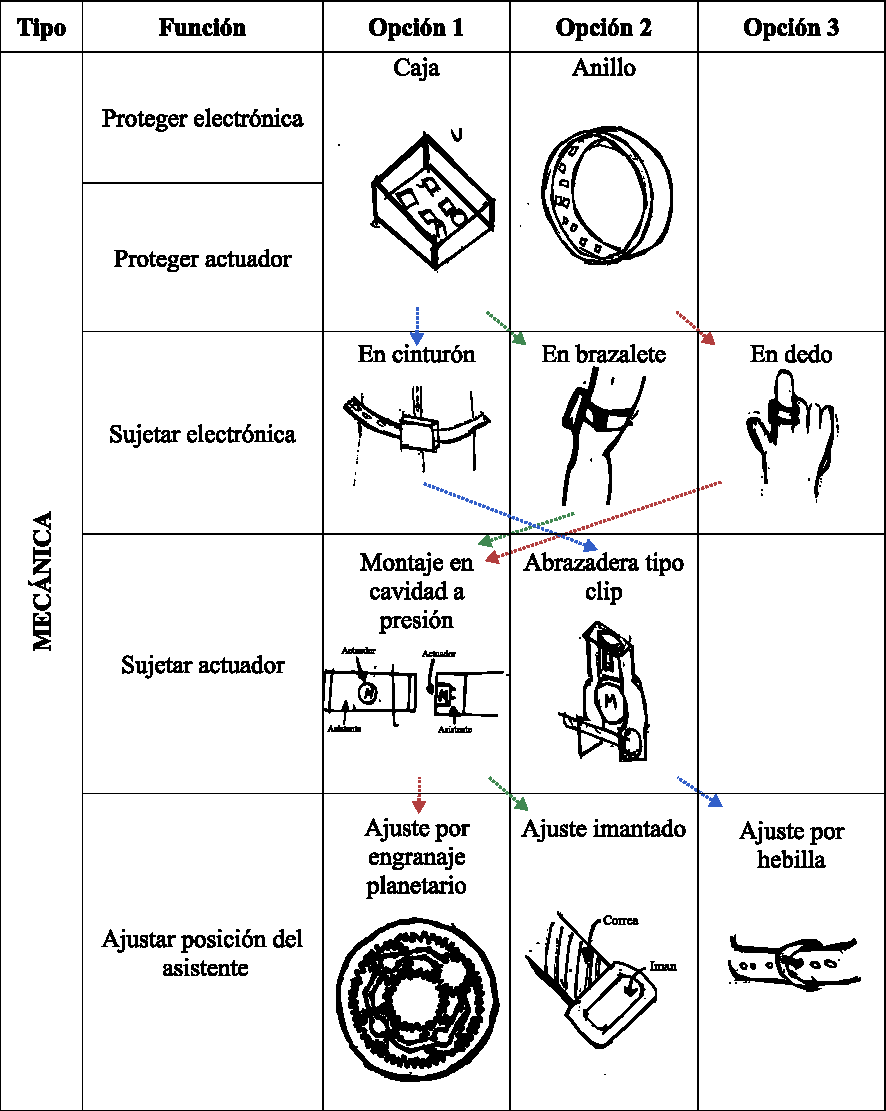
\includegraphics[width=0.8\textwidth]{CHPTRS/CH03_DICON/fig_matriz/Matriz mecanica .pdf}
\end{table}
\end{itemize}

\section{Conceptos de solución}
A continuación, se presentan tres conceptos de solución que están desarrolladas en base a las posibles combinaciones de alternativas definidas en la matriz morfológica. Posteriormente, se realiza un análisis técnico-económico para evaluar cual de estas propuestas representa la solución óptima.

\subsection{Concepto de solución 1 - Anillo}
El primer concepto solución, tiene la forma de un anillo inteligente como se puede apreciar en la Figura~\ref{fig:d.conceptual1}. El anillo cuenta con un sistema de engranaje planetario que permitirá la rotación del módulo que contiene el sensor. Así, al estar posicionado en una zona óptima para la detección de la señal, asegura una correcta lectura fisiológica. Posteriormente, esta señal pasará por una etapa de amplificación y filtración que facilitará su análisis en frecuencia. La electrónica interna se distribuye sobre una placa de circuito flexible que permite aprovechar el perímetro circular del asistente sin incomodar al usuario. En esta placa se ubicará el microcontrolador nRF534, un motor de vibración, un regulador de voltaje, el sensor fisiológico (pulsioxímetro) y una batería Li-Ion. Para garantizar el contacto entre el sensor y la piel, la parte baja del anillo contará con una ventana de lectura. Asimismo, el motor de vibración se activa a través de una señal PWM emitida por el microcontrolador cuando se detecta un estado de distracción, brindando una retroalimentación directa al usuario. Este estado de concentración o distracción es resultado del clasificador \textit{machine learning}. En adición a esto, el usuario será capaz de visualizar estadísticas, estados de concentración y podrá establecer la duración de las sesiones de estudio en una interfaz en un celular.\\

\begin{figure}[H]
\centering
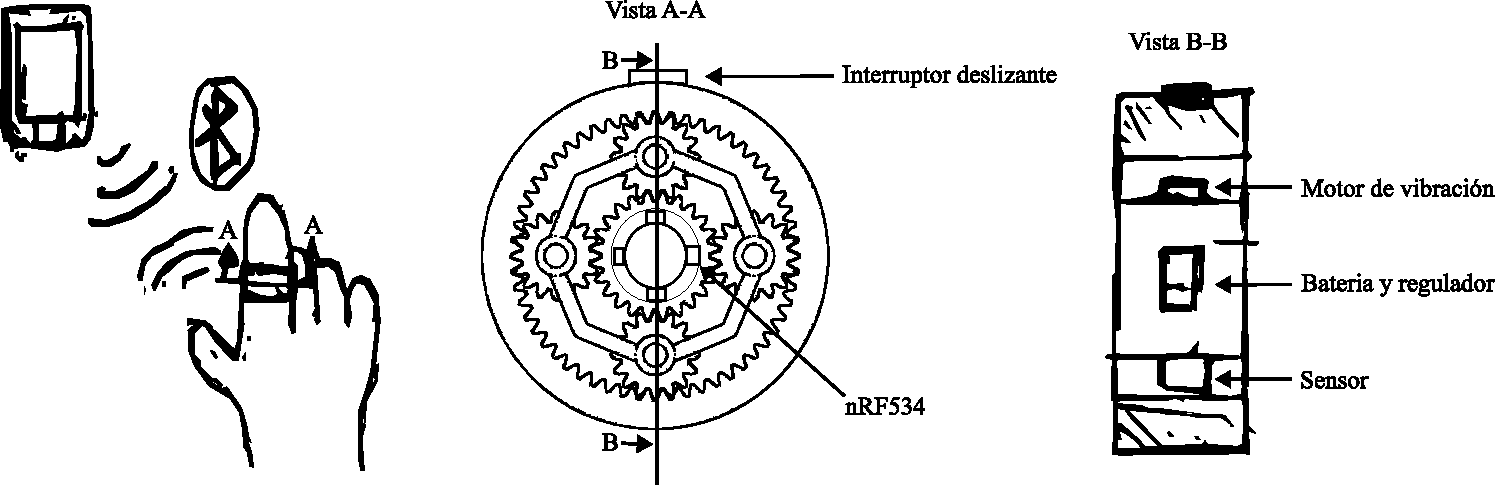
\includegraphics[width=0.9\textwidth]{CHPTRS/CH03_DICON/fig_conceptos/Conceptos de Solucion1.pdf}
\caption{Concepto de Solución 1}
\label{fig:d.conceptual1}
\captionsetup{justification=centering,margin=2cm}
%\caption*{\textit{Elaboración propia}}
\end{figure}


\subsection{Concepto de solución 2 - Banda braquial}
El segundo concepto de solución (ver Figura~\ref{fig:d.conceptual2}) consiste en un asistente en forma de pulsera, diseñada para ser usada alrededor del brazo. La correa incorpora un sistema de cierre magnético que permite un ajuste preciso. Asimismo, la batería Li-Po, el microcontrolador ESP32-C3, el regulador de voltaje, el motor de vibración, el sensor de pulso cardíaco y el amplificador operacional están contenidos en una carcasa rígida central en forma de caja, sostenida por la correa mencionada. Además, para garantizar una lectura confiable, la carcasa cuenta con un orificio en la parte central inferior, a través del cual el sensor mantiene contacto directo con la piel del brazo donde se captará la señal fisiológica que pasará por una etapa de amplificación y filtrado antes del análisis estadístico. Por otro lado, la retroalimentación se obtendrá a partir del motor de vibración al determinar un estado de distracción través de la activación de una señal PWM del microcontrolador. Este estado es el resultado del clasificador basado en aprendizaje automático. Por último, se debe mencionar que el usuario podrá establecer la duración de la sesión de estudio y visualizar sus estadísticas a través de una interfaz en un dispositivo móvil.\\

\begin{figure}[H]
\centering
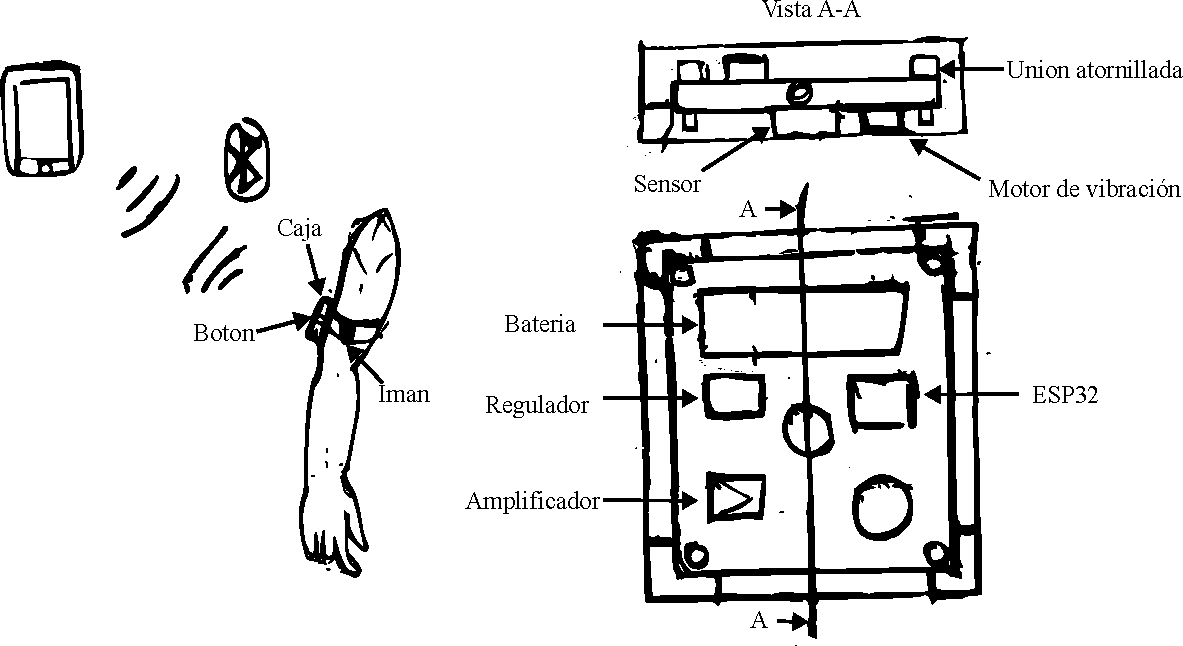
\includegraphics[width=0.8\textwidth]{CHPTRS/CH03_DICON/fig_conceptos/Conceptos de Solucion2.pdf}
\caption{Concepto de Solución 2}
\label{fig:d.conceptual2}
\captionsetup{justification=centering,margin=2cm}
%\caption*{\textit{Elaboración propia}}
\end{figure}

\subsection{Concepto de solución 3 - Cinturón}
El tercer concepto de solución consiste en un asistente en forma de cinturón, diseñado para colocarse alrededor de la parte baja del torso como se puede apreciar en la Figura~\ref{fig:d.conceptual3}. Los componentes electrónicos como la batería NiMh, el microcontrolador DA14531, el regulador, el zumbador piezoeléctrico y el sensor estarán contenidos en una carcasa paralelepípeda, la  cual estará sostenida por la correa con ajuste por hebilla. En este caso, se utiliza un acelerómetro para monitorizar la frecuencia respiratoria a través de los movimientos del abdomen. La señal del sensor varía con los movimientos rítmicos de la respiración y es enviada a una etapa de amplificación y filtrado para su posterior análisis estadístico. En caso de detectarse un estado de distracción, el sistema activa una retroalimentación por del zumbador piezoeléctrico  a través de una señal digital ON/OFF por el microcontrolador. Asimismo, el usuario puede establecer la duración de la sesión y visualizar sus resultados mediante una interfaz gráfica en una computadora.

\begin{figure}[H]
\centering
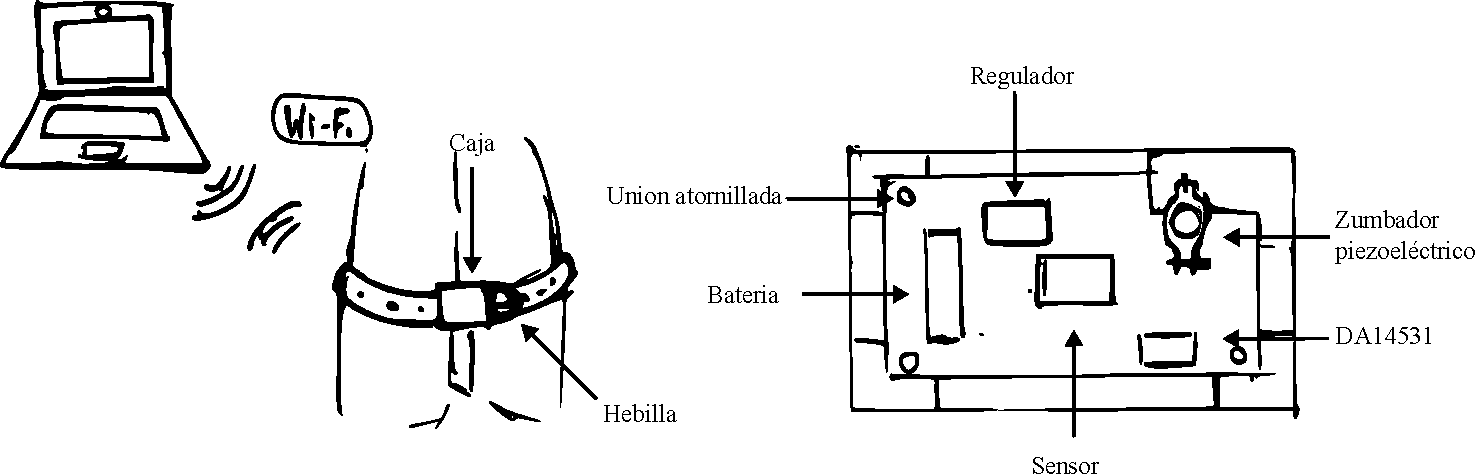
\includegraphics[width=0.8\textwidth]{CHPTRS/CH03_DICON/fig_conceptos/Conceptos de Solucion3.pdf}
\caption{Concepto de Solución 3}
\label{fig:d.conceptual3}
\captionsetup{justification=centering,margin=2cm}
%\caption*{\textit{Elaboración propia}}
\end{figure}

\section{Evaluación técnico-económica}
\label{sc:CH03-ev_tec-eco}

    En esta sección, se realiza la evaluación técnico-económica para cada concepto de solución bajo la metodología VDI 2225, la cual permite tomar decisiones objetivas en el proceso de diseño. Para ello, se realizan dos tablas, una donde se desarrolla el análisis técnico, y otra donde se muestra la evaluación económica, ver Tabla~\ref{tab:E.Tecnica} y Tabla~\ref{tab:E.Economica} respectivamente. En ambas, se asignan criterios con diferente peso en función de su importancia y a cada criterio se le asigna puntaje. Luego, el puntaje de cada solución es comparado con el puntaje ideal, lo que permite determinar cuál es la alternativa que representa la solución óptima. Para ello, se establece la leyenda que se empleará en la siguientes tablas. \\

    \hspace{-0.7cm}\underline{Leyenda:}
    
    \begin{itemize}
    \item  Puntaje $pX$, donde $X \in \mathbb{N} = \{0, 1, 2, 3, 4\}$ (Escala de Valores según VDI 2225) y se establece: 4 = Excelente,3 = Bien, 2 = Suficiente, 1 = Apenas satisface, 0 = No satisface. 
    \item Peso ponderado $qX$, donde $X \in \mathbb{N} = \{0, 1, 2, 3, 4\}$ en función de la importancia de los criterios de evaluación y se establece: 4 = muy importante, 3 = importante, 2 = poco importante, 1 = apenas importante, 0 = no importante.
    \end{itemize}
    
    
    
\subsection{Evaluación técnica}

Para realizar la evaluación técnica de los conceptos de solución se han definido ocho criterios fundamentales como se puede apreciar en la Tabla ~\ref{tab:E.Tecnica}. El primero es la función principal, que valora la capacidad para cumplir el objetivo de detectar y reducir la distracción. El criterio de  forma considera que tan compacto es el asistente y su portabilidad. La ergonomía evalúa el nivel de comodidad que puede llegar a ofrecer el asistente considerando su tamaño. Asimismo, la viabilidad del algoritmo analiza la posibilidad de implementar el algoritmo y su precisión. Por el lado del criterio energía, esta evalúa la autonomía del sistema. Finalmente, los criterios de fabricación y mantenimiento valoran la facilidad de integración y la posibilidad de realizar reparaciones en caso de fallos. En este caso, los resultados determinan que el concepto solución 1 es el que tiene mayor valor técnico, el cual es representado en la variable $Xi$.\\

    \hspace{-0.7cm}\underline{Justificación de puntuación por criterio:}
    
    \begin{itemize}
    \item Función Principal: considerando que los tres conceptos solución están enfocados en cumplir la función principal, se les asigna el mismo puntaje en este criterio.
    \item Forma: en este caso se consideró p4 al \ac{CoS}-1 por su alta portabilidad y lo compacto que es al ser un anillo , p3 al segundo concepto por tener una portabilidad mediana al ser una banda braquial y p2 al tercero, ya que al ser un cinturón tiene una menor portabilidad debido al largo de la correa.
    \item Ergonomía: tanto el primer concepto solución como el segundo tienen un p3 debido a que presentan un tamaño reducido y su ubicación permiten un uso relativamente cómodo y poco invasivo. Por otro lado, el \ac{CoS}-3 recibe p2, ya que, al tratarse de un cinturón, puede generar incomodidad o restricción en la zona abdominal.
    \item Viabilidad algoritmo: el \ac{CoS}-1 obtiene p4 debido a que esta pensado a realizarse con análisis en frecuencia y un clasificador \textit{machine learning}, lo que representa un enfoque avanzado y robusto. Asimismo, el segundo p3 porque, si bien también utiliza un clasificador, se realiza un análisis estadístico en lugar de uno de frecuencia. El tercero un p2 porque utiliza umbral dinámico y estadística, lo que implica menor complejidad y precisión.
    \item Energía: todos los conceptos de solución están pensados para ofrecer autonomía a través de las baterías y un consumo energético no elevado. Por ello, se le asigna un puntaje de 3 de forma uniforme.
    \item Seguridad: los conceptos de solución ofrecen la misma seguridad, ya que por la posición y la forma de estos, evitan que el usuario sufra algún daño. Así, los 3 conceptos tienen un puntaje p3.
    \item Fabricación: los tres conceptos de solución presentan una dificultad de fabricación similar, ya que se busca que sea lo más compacto posible. Sin embargo, el primero cuenta con un sistema planetario de engranajes en un espacio limitado, lo que dificulta su fabricación. Por ello, se le asigna un puntaje menor que al resto de conceptos.
    \item Mantenimiento: el primer concepto de solución, al ser un anillo, tiene un espacio muy reducido y los componentes deberán estar altamente compactados, lo que dificulta considerablemente su mantenimiento, por lo que se asigna un p1. Por otro lado, tanto el segundo como el tercer concepto de solución, presentan un p3, ya que al tener los componentes dentro de una carcasa, permiten un mantenimiento más sencillo.
    \end{itemize}


\begin{table}[H]
    \centering
    \caption{Evaluación técnica}
    \label{tab:E.Tecnica}
    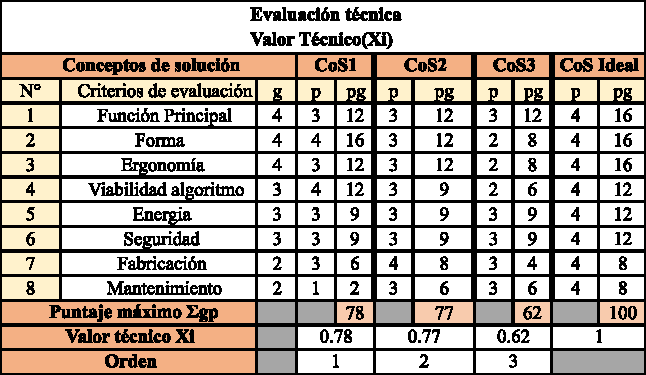
\includegraphics[width=0.8\textwidth]{CHPTRS/CH03_DICON/fig_conceptos/Evaluación técnica.pdf}
\end{table}

\subsection{Evaluación económica}
La evaluación económica determina el concepto de solución más viable en términos de costos a través de los cuatro criterios establecidos como se muestra en la Tabla~\ref{tab:E.Economica}. El primer criterio  es el costo de materiales, que hace referencia al precio de los componentes electrónicos y mecánicos necesarios para implementar el asistente. El criterio de repuesto de piezas evalúa la facilidad de sustitución y el costo asociado a la sustitución de componentes en caso de fallos. En el caso de costo de fabricación se considera los recursos económicos para el ensamblado del asistente. Finalmente, el costo de mantenimiento estima los gastos asociados al uso prologando del asistente y posibles intervenciones a lo largo de su vida útil, tales como reemplazo de componentes electrónicos, correa en caso del \ac{CoS}-2 o el sistema planetario del \ac{CoS}-1. Asimismo, para realizar la asignación de los puntajes se realizo una lista de precios preliminar teniendo en cuenta solo los componentes electrónicos más importantes de cada concepto solución, donde se aprecian los precisos por unidad para los repuestos y al por mayor para producción, estas tablas se pueden encontrar en el \hyperref[an:Annex_D_precios_preliminares]{Anexo D}. Los resultados de esta evaluación determinan que el concepto solución 3 es aquel con mayor valor económico, el cual es representado en la variable $Yi$.

\begin{table}[H]
    \centering
    \caption{Evaluación Económica}
    \label{tab:E.Economica}
    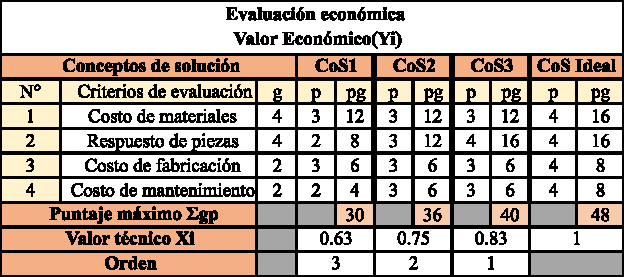
\includegraphics[width=0.8\textwidth]{CHPTRS/CH03_DICON/fig_conceptos/Evaluación economica.pdf}
\end{table}

Se muestra en la Figura~\ref{fig:tecnico-economico}, el análisis técnico-económico para determinar el concepto de solución óptimo con los resultados de las tablas anteriores. El concepto óptimo es aquel que se encuentre a la menor distancia a la recta con pendiente equivalente a la unidad de la solución ideal. Se puede apreciar con facilidad que el \ac{CoS}-2 se encuentra muy cerca de la solución ideal, siendo este el ganador.\\

\begin{figure}[H]
\centering
\begin{center}
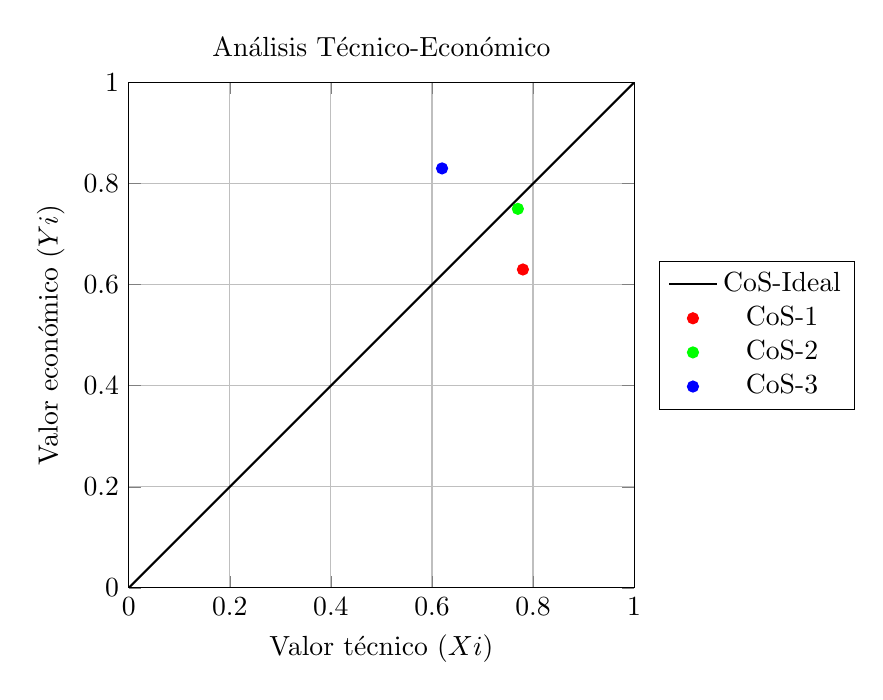
\begin{tikzpicture}
\begin{axis}[
    title={Análisis Técnico-Económico},
    xlabel={Valor técnico ($Xi$)},
    ylabel={Valor económico ($Yi$)},
    xmin=0, xmax=1,
    ymin=0, ymax=1,
    grid=both,
    legend style={at={(1.05,0.5)}, anchor=west},
    width=12cm,
    height=8cm,
    axis equal image,
    scatter/classes={
        CS-1={mark=*,red},
        CS-2={mark=*,green},
        CS-3={mark=*,blue}
    }
]

% Línea de referencia (línea diagonal)
\addplot[domain=0:1, color=black, thick] {x};

% Puntos
\addplot[
    scatter,
    only marks,
    scatter src=explicit symbolic
] coordinates {
    (0.78,0.63) [CS-1]
    (0.77,0.75) [CS-2]
    (0.62,0.83) [CS-3]
};

\legend{CoS-Ideal,CoS-1, CoS-2, CoS-3}

\end{axis}
\end{tikzpicture}
\end{center}
\caption{Análisis técnico-económico}
\label{fig:tecnico-economico}
\captionsetup{justification=centering,margin=2cm}
%\caption*{\textit{Elaboración propia}}
\end{figure}

\section{Concepto de Solución óptimo}

En la sección \hyperref[sc:CH03-ev_tec-eco]{3.5} se demostró que el \ac{CoS}-2 es la solución óptima. Este corresponde a un asistente en forma de banda braquial, diseñado para ser colocado alrededor del brazo del usuario, ligeramente por encima del bíceps. Esta solución ofrece un equilibrio entre portabilidad, comodidad y espacio suficiente para albergar los componentes electrónicos necesarios. \\

La solución óptima se compone de una correa ajustable como se puede apreciar en la Figura~\ref{fig:SolucionOptima} mediante un sistema magnético, asegurando un agarre preciso y justo que se puede adaptar a distintos tamaños de brazo. Asimismo, cuenta con una carcasa rígida de forma paralelepípeda que deberá tener los bordes redondeados por seguridad. Además, esta carcasa contiene los componentes electrónicos: microcontrolador, batería, regulador de voltaje, sensor de pulso cardíaco y motor de vibración para la retroalimentación. Estos estarán en una placa de circuito impreso fijada a la carcasa mediante uniones atornilladas dentro de la carcasa.  \\

Para garantizar la fiabilidad en la captura de la señal fisiológica, la carcasa cuenta con una apertura que permite el contacto directo entre el sensor y la piel del usuario. La señal captada es procesada en el asistente y, en caso de detectarse un estado de distracción, se genera una vibración como retroalimentación inmediata. Además, mediante comunicación inalámbrica \textit{bluetooth}, se envían los datos de concentración al aplicativo móvil, donde el usuario puede visualizar sus estadísticas y configurar la duración de las sesiones de estudio.\\

Esta solución destaca por su ergonomía, facilidad de uso y la adecuada ubicación del sensor, lo que permite una lectura confiable sin comprometer la comodidad del usuario. Asimismo, su tamaño intermedio facilita la integración de los componentes electrónicos, lo que permite simplificar su fabricación y mantenimiento.\\

\begin{figure}[H]
\centering
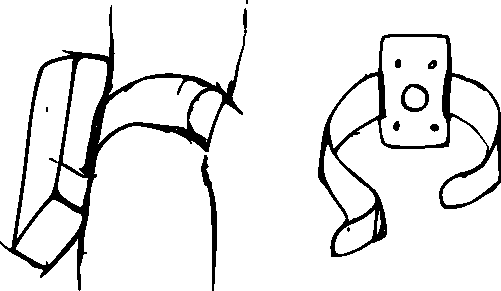
\includegraphics[width=0.7\textwidth]{CHPTRS/CH03_DICON/fig_conceptos/Concepto optimo.pdf}
\caption{Solución óptima}
\label{fig:SolucionOptima}
\captionsetup{justification=centering,margin=1cm}
%\caption*{\textit{Elaboración propia}}
\end{figure}


\subsection{Diagrama de flujo general}

Se presenta el diagrama de flujo general del asistente propuesto a nivel de microcontrolador en la Figura~\ref{fig:diagramaDeFlujo}, el cual describe de manera secuencial el funcionamiento lógico del sistema. El proceso inicia con el encendido del dispositivo mediante un botón, seguido de la configuración de la duración de la sesión de estudio por parte del usuario. Posteriormente, el asistente procede a captar la señal fisiológica, la cual es procesada y analizada para determinar el nivel de concentración del usuario. Esta información es enviada al aplicativo móvil y en caso de que sea distracción se activa la retroalimentación. Esto se repite de forma continua hasta que la sesión de estudio es finalizada.\\

Asimismo, en la Figura~\ref{fig:diagramaDeFlujoApp} se muestra el diagrama de flujo general a nivel del aplicativo móvil. El proceso inicia con la visualización de la pantalla inicial. Luego, se establece la conexión \textit{blueetooth} con el asistente; en caso de fallo de conexión, se muestra un mensaje indicatorio y se repite el proceso. Una vez establecida la conexión, el usuario puede configurar la duración de la sesión de estudio. Posteriormente, el aplicativo permanece en estado de monitoreo en tiempo real, donde en caso de recibir datos, se muestra el estado de concentración y las estadísticas del usuario hasta que la sesión finaliza. En caso de que no se reciban datos durante el monitoreo, se muestra una alerta de pérdida de conexión al usuario. 

\begin{figure}[H]
\centering
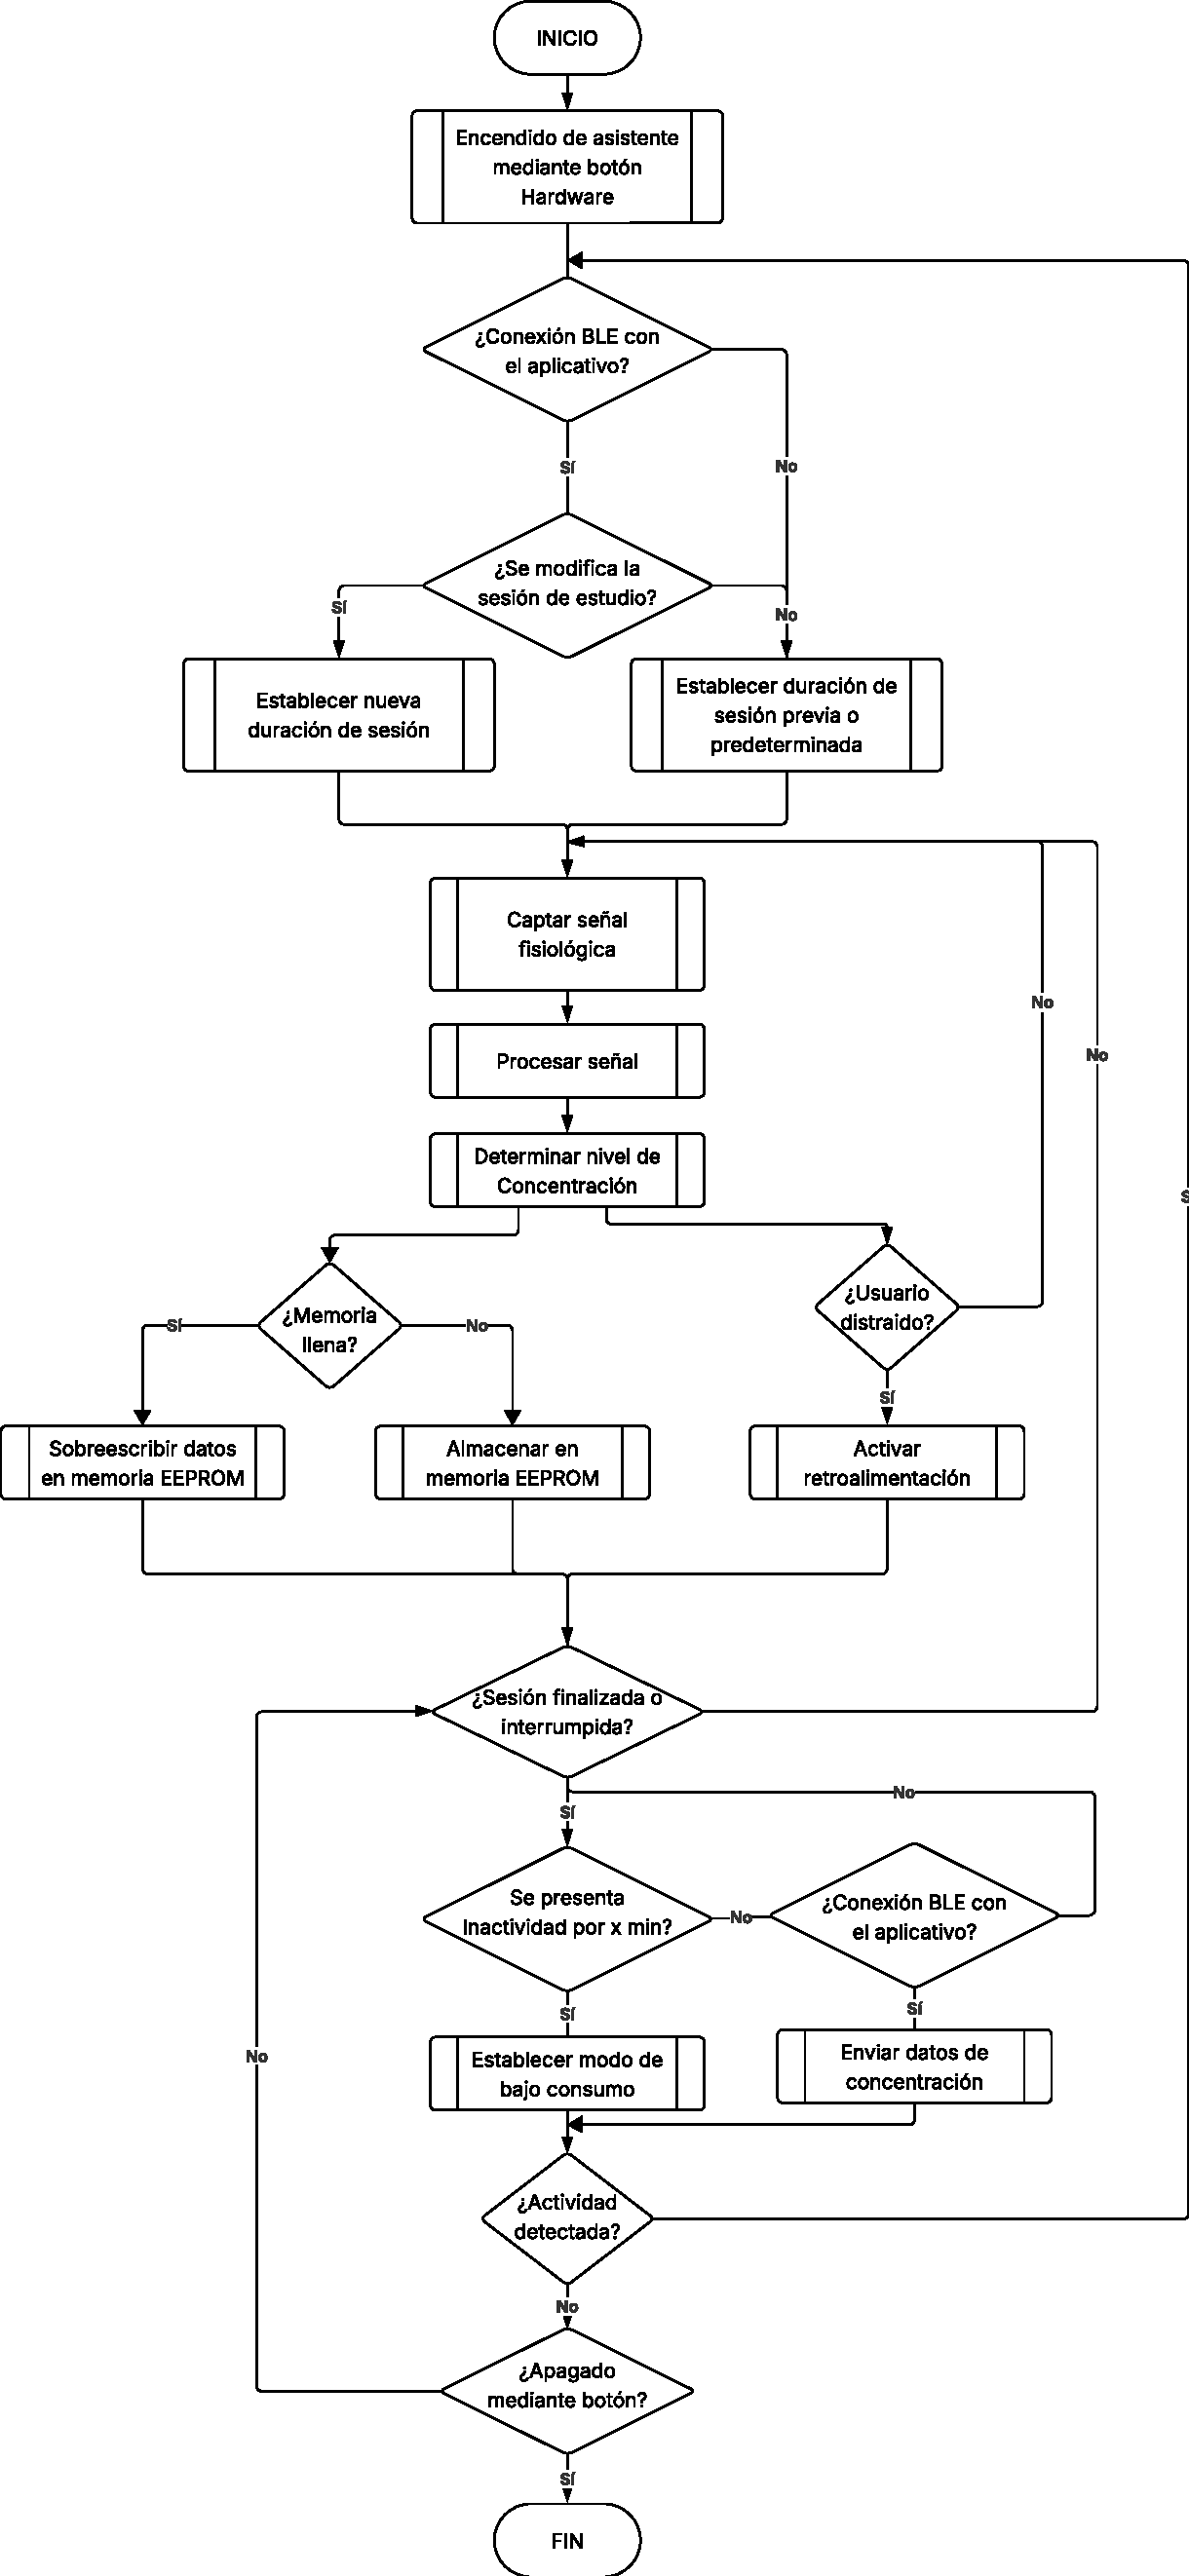
\includegraphics[width=0.63\textwidth]{CHPTRS/CH03_DICON/fig_conceptos/Daigramas de Flujo TESIS.pdf}
\caption{Diagrama de flujo general del microcontrolador}
\label{fig:diagramaDeFlujo}
\captionsetup{justification=centering,margin=1cm}
%\caption*{\textit{Elaboración propia}}
\end{figure}

\begin{figure}[H]
\centering
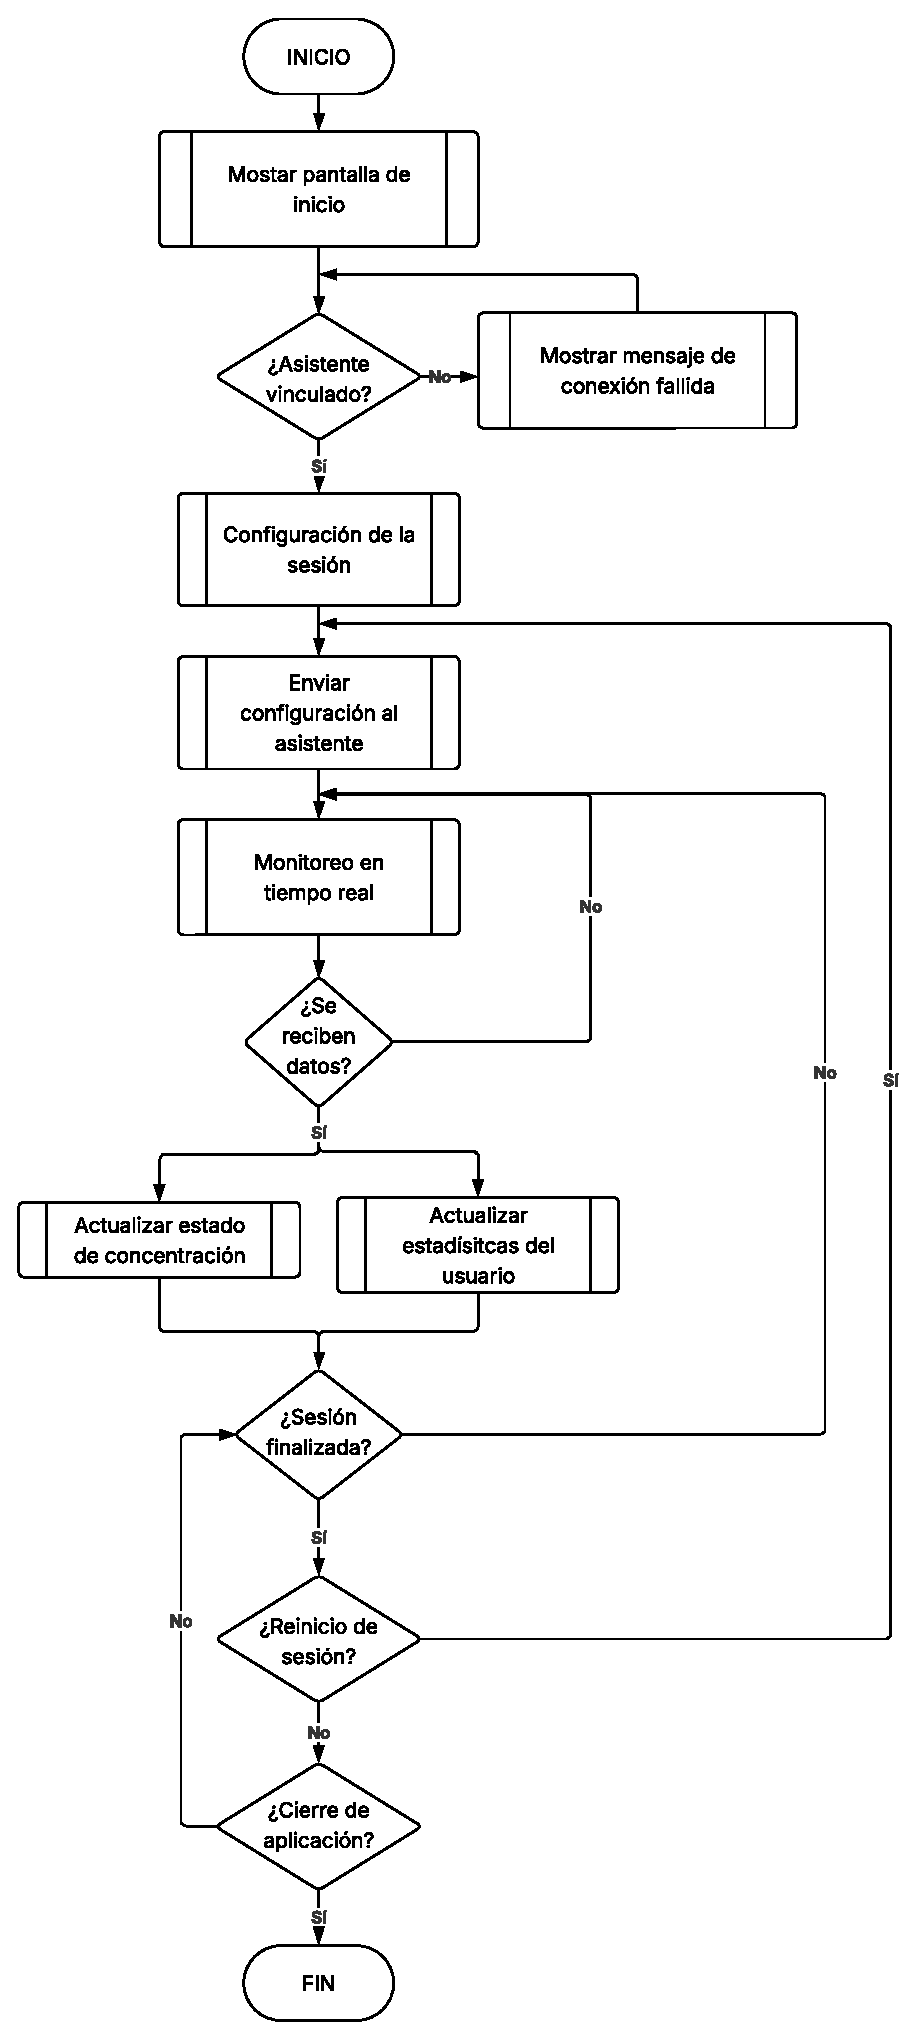
\includegraphics[width=0.6\textwidth]{CHPTRS/CH03_DICON/fig_conceptos/Daigramas de Flujo Aplicativo.pdf}
\caption{Diagrama de flujo general del aplicativo}
\label{fig:diagramaDeFlujoApp}
\captionsetup{justification=centering,margin=1cm}
%\caption*{\textit{Elaboración propia}}
\end{figure}
\cleardoublepage
\subsection{Diagrama de máquina de estados general}
La Figura~\ref{fig:maquinaDEstadoGeneral} muestra el diagrama de la máquina de estados general que rige el funcionamiento del asistente. Este representa los diferentes estados en los que se puede encontrar el dispositivo, así como las transiciones que se producen en función de las acciones del usuario y los eventos internos del sistema. El estado inicial corresponde al encendido del sistema  y prosigue con la recepción de la configuración de la sesión. Posteriormente, el asistente puede pasar al modo de reposo IDLE o al estado de monitoreo dependiendo si hay sesión activa. En el estado de monitoreo se incluye el procesamiento de la señal, así como la transmisión de datos y la activación del estado de retroalimentación, en el cual se genera una vibración para alertar al usuario. Una vez que finalice la sesión de estudio, el sistema retorna al estado de reposo o en caso de que se presione el botón durante cualquiera de los otros estados al apagado del sistema.

\begin{figure}[H]
\centering
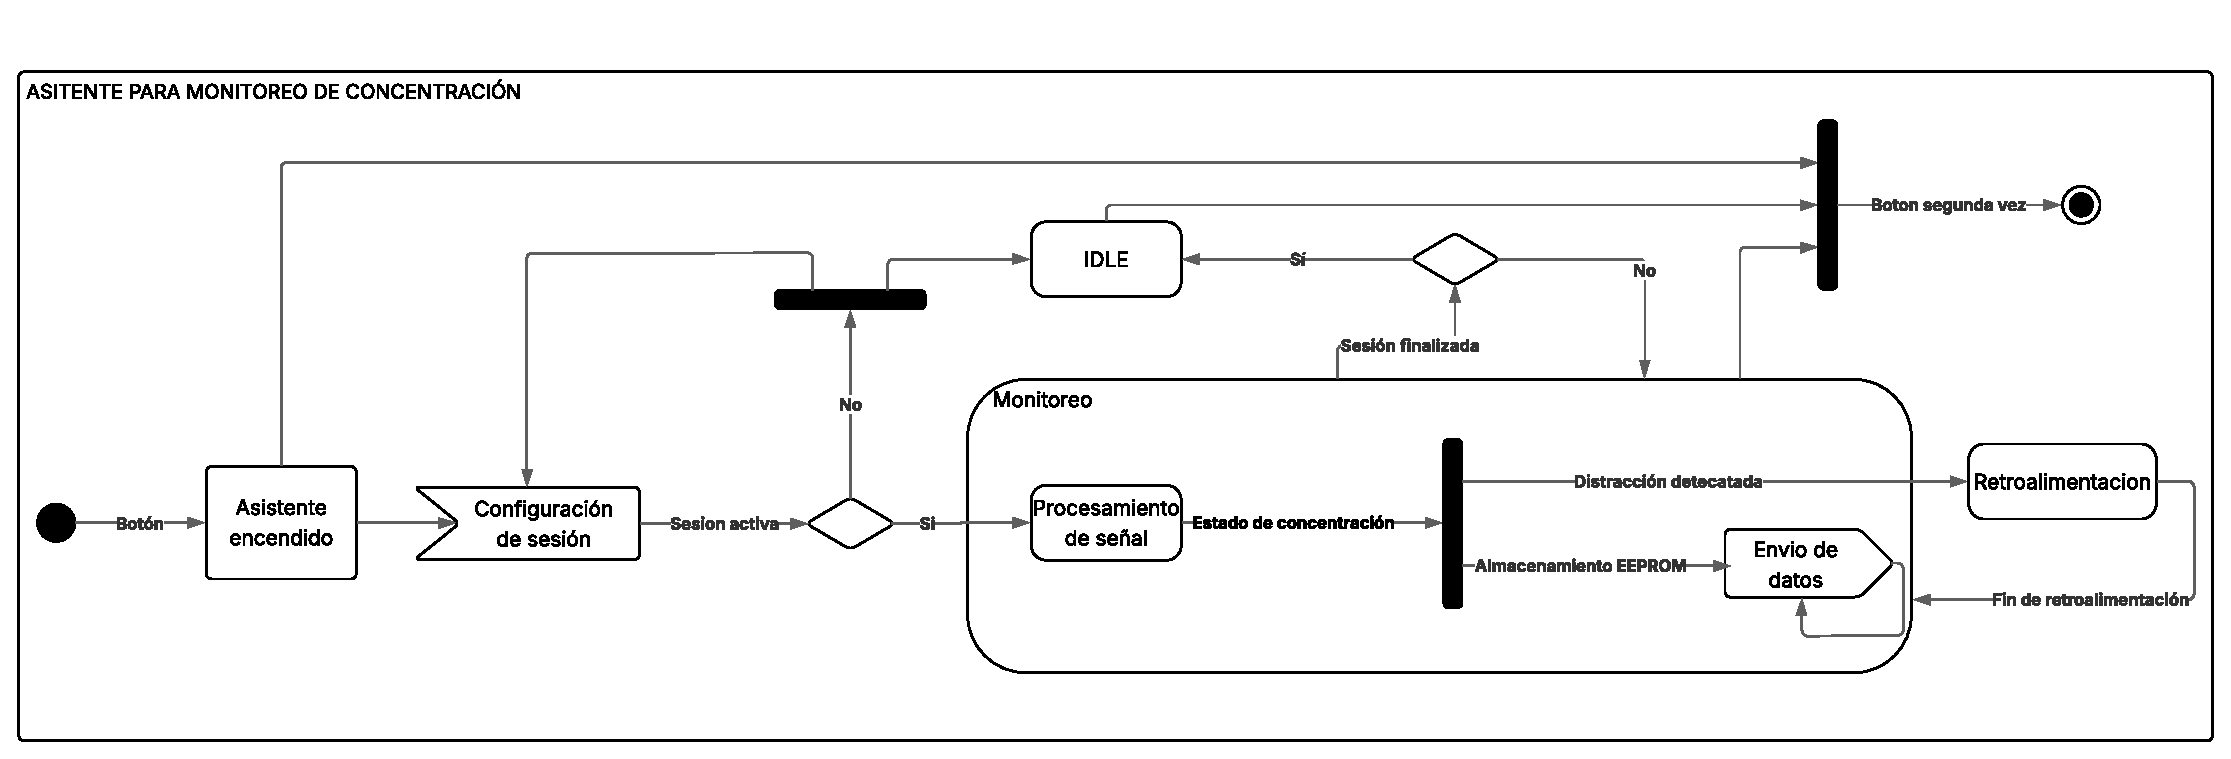
\includegraphics[width=1\textwidth]{CHPTRS/CH03_DICON/fig_conceptos/Maquina estados.pdf}
\caption{Diagrama de máquina de estados general}
\label{fig:maquinaDEstadoGeneral}
\captionsetup{justification=centering,margin=1cm}
%\caption*{\textit{Elaboración propia}}
\end{figure}










